\documentclass[]{book}
\usepackage{lmodern}
\usepackage{amssymb,amsmath}
\usepackage{ifxetex,ifluatex}
\usepackage{fixltx2e} % provides \textsubscript
\ifnum 0\ifxetex 1\fi\ifluatex 1\fi=0 % if pdftex
  \usepackage[T1]{fontenc}
  \usepackage[utf8]{inputenc}
\else % if luatex or xelatex
  \ifxetex
    \usepackage{mathspec}
  \else
    \usepackage{fontspec}
  \fi
  \defaultfontfeatures{Ligatures=TeX,Scale=MatchLowercase}
\fi
% use upquote if available, for straight quotes in verbatim environments
\IfFileExists{upquote.sty}{\usepackage{upquote}}{}
% use microtype if available
\IfFileExists{microtype.sty}{%
\usepackage{microtype}
\UseMicrotypeSet[protrusion]{basicmath} % disable protrusion for tt fonts
}{}
\usepackage{hyperref}
\hypersetup{unicode=true,
            pdftitle={Spatial Analysis Notes},
            pdfauthor={Francisco Rowe-Gonzalez \& Dani Arribas-Bel},
            pdfborder={0 0 0},
            breaklinks=true}
\urlstyle{same}  % don't use monospace font for urls
\usepackage{natbib}
\bibliographystyle{apalike}
\usepackage{color}
\usepackage{fancyvrb}
\newcommand{\VerbBar}{|}
\newcommand{\VERB}{\Verb[commandchars=\\\{\}]}
\DefineVerbatimEnvironment{Highlighting}{Verbatim}{commandchars=\\\{\}}
% Add ',fontsize=\small' for more characters per line
\usepackage{framed}
\definecolor{shadecolor}{RGB}{248,248,248}
\newenvironment{Shaded}{\begin{snugshade}}{\end{snugshade}}
\newcommand{\AlertTok}[1]{\textcolor[rgb]{0.94,0.16,0.16}{#1}}
\newcommand{\AnnotationTok}[1]{\textcolor[rgb]{0.56,0.35,0.01}{\textbf{\textit{#1}}}}
\newcommand{\AttributeTok}[1]{\textcolor[rgb]{0.77,0.63,0.00}{#1}}
\newcommand{\BaseNTok}[1]{\textcolor[rgb]{0.00,0.00,0.81}{#1}}
\newcommand{\BuiltInTok}[1]{#1}
\newcommand{\CharTok}[1]{\textcolor[rgb]{0.31,0.60,0.02}{#1}}
\newcommand{\CommentTok}[1]{\textcolor[rgb]{0.56,0.35,0.01}{\textit{#1}}}
\newcommand{\CommentVarTok}[1]{\textcolor[rgb]{0.56,0.35,0.01}{\textbf{\textit{#1}}}}
\newcommand{\ConstantTok}[1]{\textcolor[rgb]{0.00,0.00,0.00}{#1}}
\newcommand{\ControlFlowTok}[1]{\textcolor[rgb]{0.13,0.29,0.53}{\textbf{#1}}}
\newcommand{\DataTypeTok}[1]{\textcolor[rgb]{0.13,0.29,0.53}{#1}}
\newcommand{\DecValTok}[1]{\textcolor[rgb]{0.00,0.00,0.81}{#1}}
\newcommand{\DocumentationTok}[1]{\textcolor[rgb]{0.56,0.35,0.01}{\textbf{\textit{#1}}}}
\newcommand{\ErrorTok}[1]{\textcolor[rgb]{0.64,0.00,0.00}{\textbf{#1}}}
\newcommand{\ExtensionTok}[1]{#1}
\newcommand{\FloatTok}[1]{\textcolor[rgb]{0.00,0.00,0.81}{#1}}
\newcommand{\FunctionTok}[1]{\textcolor[rgb]{0.00,0.00,0.00}{#1}}
\newcommand{\ImportTok}[1]{#1}
\newcommand{\InformationTok}[1]{\textcolor[rgb]{0.56,0.35,0.01}{\textbf{\textit{#1}}}}
\newcommand{\KeywordTok}[1]{\textcolor[rgb]{0.13,0.29,0.53}{\textbf{#1}}}
\newcommand{\NormalTok}[1]{#1}
\newcommand{\OperatorTok}[1]{\textcolor[rgb]{0.81,0.36,0.00}{\textbf{#1}}}
\newcommand{\OtherTok}[1]{\textcolor[rgb]{0.56,0.35,0.01}{#1}}
\newcommand{\PreprocessorTok}[1]{\textcolor[rgb]{0.56,0.35,0.01}{\textit{#1}}}
\newcommand{\RegionMarkerTok}[1]{#1}
\newcommand{\SpecialCharTok}[1]{\textcolor[rgb]{0.00,0.00,0.00}{#1}}
\newcommand{\SpecialStringTok}[1]{\textcolor[rgb]{0.31,0.60,0.02}{#1}}
\newcommand{\StringTok}[1]{\textcolor[rgb]{0.31,0.60,0.02}{#1}}
\newcommand{\VariableTok}[1]{\textcolor[rgb]{0.00,0.00,0.00}{#1}}
\newcommand{\VerbatimStringTok}[1]{\textcolor[rgb]{0.31,0.60,0.02}{#1}}
\newcommand{\WarningTok}[1]{\textcolor[rgb]{0.56,0.35,0.01}{\textbf{\textit{#1}}}}
\usepackage{longtable,booktabs}
\usepackage{graphicx,grffile}
\makeatletter
\def\maxwidth{\ifdim\Gin@nat@width>\linewidth\linewidth\else\Gin@nat@width\fi}
\def\maxheight{\ifdim\Gin@nat@height>\textheight\textheight\else\Gin@nat@height\fi}
\makeatother
% Scale images if necessary, so that they will not overflow the page
% margins by default, and it is still possible to overwrite the defaults
% using explicit options in \includegraphics[width, height, ...]{}
\setkeys{Gin}{width=\maxwidth,height=\maxheight,keepaspectratio}
\IfFileExists{parskip.sty}{%
\usepackage{parskip}
}{% else
\setlength{\parindent}{0pt}
\setlength{\parskip}{6pt plus 2pt minus 1pt}
}
\setlength{\emergencystretch}{3em}  % prevent overfull lines
\providecommand{\tightlist}{%
  \setlength{\itemsep}{0pt}\setlength{\parskip}{0pt}}
\setcounter{secnumdepth}{5}
% Redefines (sub)paragraphs to behave more like sections
\ifx\paragraph\undefined\else
\let\oldparagraph\paragraph
\renewcommand{\paragraph}[1]{\oldparagraph{#1}\mbox{}}
\fi
\ifx\subparagraph\undefined\else
\let\oldsubparagraph\subparagraph
\renewcommand{\subparagraph}[1]{\oldsubparagraph{#1}\mbox{}}
\fi

%%% Use protect on footnotes to avoid problems with footnotes in titles
\let\rmarkdownfootnote\footnote%
\def\footnote{\protect\rmarkdownfootnote}

%%% Change title format to be more compact
\usepackage{titling}

% Create subtitle command for use in maketitle
\providecommand{\subtitle}[1]{
  \posttitle{
    \begin{center}\large#1\end{center}
    }
}

\setlength{\droptitle}{-2em}

  \title{Spatial Analysis Notes}
    \pretitle{\vspace{\droptitle}\centering\huge}
  \posttitle{\par}
    \author{Francisco Rowe-Gonzalez \& Dani Arribas-Bel}
    \preauthor{\centering\large\emph}
  \postauthor{\par}
      \predate{\centering\large\emph}
  \postdate{\par}
    \date{2020-02-03}

\usepackage{booktabs}
\usepackage{amsthm}
\makeatletter
\def\thm@space@setup{%
  \thm@preskip=8pt plus 2pt minus 4pt
  \thm@postskip=\thm@preskip
}
\makeatother

\begin{document}
\maketitle

{
\setcounter{tocdepth}{1}
\tableofcontents
}
\hypertarget{spatial-analysis-notes}{%
\chapter{Spatial Analysis Notes}\label{spatial-analysis-notes}}

{[}Introduction here{]}

\hypertarget{intro}{%
\chapter{Introduction}\label{intro}}

FR-G to fill in

\hypertarget{points}{%
\chapter{Points}\label{points}}

This session\footnote{This note is part of \href{index.html}{Spatial Analysis Notes} {Points -- Kernel Density Estimation and Spatial interpolation} by Dani Arribas-Bel is licensed under a Creative Commons Attribution-NonCommercial-ShareAlike 4.0 International License.} is based on the following references, which are great follow-up's on the topic:

\begin{itemize}
\tightlist
\item
  \citet{lovelace2014introduction} is a great introduction.
\item
  Chapter 6 of \citet{comber2015}, in particular subsections 6.3 and 6.7.
\item
  \citet{bivand2013applied} provides an in-depth treatment of spatial data in R.
\end{itemize}

This tutorial is part of \href{index.html}{Spatial Analysis Notes}, a compilation hosted as a GitHub repository that you can access it in a few ways:

\begin{itemize}
\tightlist
\item
  As a \href{https://github.com/darribas/spa_notes/archive/master.zip}{download} of a \texttt{.zip} file that contains all the materials.
\item
  As an \href{http://darribas.org/spa_notes/points.html}{html
  website}.
\item
  As a \href{https://github.com/darribas/spa_notes/raw/master/points_book.pdf}{pdf
  document}
\item
  As a \href{https://github.com/darribas/spa_notes}{GitHub repository}.
\end{itemize}

\hypertarget{dependencies}{%
\section{Dependencies}\label{dependencies}}

This tutorial relies on the following libraries that you will need to have installed on your machine to be able to interactively follow along\footnote{You can install package \texttt{mypackage} by running the command \texttt{install.packages("mypackage")} on the R prompt or through the \texttt{Tools\ -\/-\textgreater{}\ Install\ Packages...} menu in RStudio.}. Once installed, load them up with the following commands:

\begin{Shaded}
\begin{Highlighting}[]
\CommentTok{# Layout}
\KeywordTok{library}\NormalTok{(tufte)}
\CommentTok{# For pretty table}
\KeywordTok{library}\NormalTok{(knitr)}
\CommentTok{# Spatial Data management}
\KeywordTok{library}\NormalTok{(rgdal)}
\end{Highlighting}
\end{Shaded}

\begin{verbatim}
## Loading required package: sp
\end{verbatim}

\begin{verbatim}
## rgdal: version: 1.4-4, (SVN revision 833)
##  Geospatial Data Abstraction Library extensions to R successfully loaded
##  Loaded GDAL runtime: GDAL 2.2.3, released 2017/11/20
##  Path to GDAL shared files: /usr/share/gdal/2.2
##  GDAL binary built with GEOS: TRUE 
##  Loaded PROJ.4 runtime: Rel. 4.9.3, 15 August 2016, [PJ_VERSION: 493]
##  Path to PROJ.4 shared files: (autodetected)
##  Linking to sp version: 1.3-1
\end{verbatim}

\begin{Shaded}
\begin{Highlighting}[]
\CommentTok{# Pretty graphics}
\KeywordTok{library}\NormalTok{(ggplot2)}
\CommentTok{# Thematic maps}
\KeywordTok{library}\NormalTok{(tmap)}
\CommentTok{# Pretty maps}
\KeywordTok{library}\NormalTok{(ggmap)}
\end{Highlighting}
\end{Shaded}

\begin{verbatim}
## Google's Terms of Service: https://cloud.google.com/maps-platform/terms/.
\end{verbatim}

\begin{verbatim}
## Please cite ggmap if you use it! See citation("ggmap") for details.
\end{verbatim}

\begin{Shaded}
\begin{Highlighting}[]
\CommentTok{# Various GIS utilities}
\KeywordTok{library}\NormalTok{(GISTools)}
\end{Highlighting}
\end{Shaded}

\begin{verbatim}
## Loading required package: maptools
\end{verbatim}

\begin{verbatim}
## Checking rgeos availability: TRUE
\end{verbatim}

\begin{verbatim}
## Loading required package: RColorBrewer
\end{verbatim}

\begin{verbatim}
## Loading required package: MASS
\end{verbatim}

\begin{verbatim}
## Loading required package: rgeos
\end{verbatim}

\begin{verbatim}
## rgeos version: 0.5-1, (SVN revision 614)
##  GEOS runtime version: 3.6.2-CAPI-1.10.2 
##  Linking to sp version: 1.3-1 
##  Polygon checking: TRUE
\end{verbatim}

\begin{Shaded}
\begin{Highlighting}[]
\CommentTok{# For all your interpolation needs}
\KeywordTok{library}\NormalTok{(gstat)}
\end{Highlighting}
\end{Shaded}

\begin{verbatim}
## Registered S3 method overwritten by 'xts':
##   method     from
##   as.zoo.xts zoo
\end{verbatim}

\begin{Shaded}
\begin{Highlighting}[]
\CommentTok{# For data manipulation}
\KeywordTok{library}\NormalTok{(plyr)}
\end{Highlighting}
\end{Shaded}

Before we start any analysis, let us set the path to the directory where we are working. We can easily do that with \texttt{setwd()}. Please replace in the following line the path to the folder where you have placed this file -and where the \texttt{house\_transactions} folder with the data lives.

\begin{Shaded}
\begin{Highlighting}[]
\CommentTok{#setwd('/media/dani/baul/AAA/Documents/teaching/u-lvl/2016/envs453/code')}
\KeywordTok{setwd}\NormalTok{(}\StringTok{'.'}\NormalTok{)}
\end{Highlighting}
\end{Shaded}

\hypertarget{data}{%
\section{Data}\label{data}}

For this session, we will use a subset of residential property transaction data for the city of Liverpool. These are provided by the Land Registry (as part of their \href{https://www.gov.uk/government/collections/price-paid-data}{Price Paid Data}) but have been cleaned and re-packaged by Dani Arribas-Bel.

Let us start by reading the data, which comes in a shapefile:

\begin{Shaded}
\begin{Highlighting}[]
\NormalTok{db <-}\StringTok{ }\KeywordTok{readOGR}\NormalTok{(}\DataTypeTok{dsn =} \StringTok{'data/house_transactions'}\NormalTok{, }\DataTypeTok{layer =} \StringTok{'liv_house_trans'}\NormalTok{)}
\end{Highlighting}
\end{Shaded}

\begin{verbatim}
## OGR data source with driver: ESRI Shapefile 
## Source: "/home/jovyan/work/data/house_transactions", layer: "liv_house_trans"
## with 6324 features
## It has 18 fields
## Integer64 fields read as strings:  price
\end{verbatim}

Before we forget, let us make sure \texttt{price} is considered a number, not a factor:

\begin{Shaded}
\begin{Highlighting}[]
\NormalTok{db}\OperatorTok{@}\NormalTok{data}\OperatorTok{$}\NormalTok{price <-}\StringTok{ }\KeywordTok{as.numeric}\NormalTok{(}\KeywordTok{as.character}\NormalTok{((db}\OperatorTok{@}\NormalTok{data}\OperatorTok{$}\NormalTok{price)))}
\end{Highlighting}
\end{Shaded}

The dataset spans the year 2014:

\begin{Shaded}
\begin{Highlighting}[]
\CommentTok{# Format dates}
\NormalTok{dts <-}\StringTok{ }\KeywordTok{as.Date}\NormalTok{(db}\OperatorTok{@}\NormalTok{data}\OperatorTok{$}\NormalTok{trans_date)}
\CommentTok{# Set up summary table}
\NormalTok{tab <-}\StringTok{ }\KeywordTok{summary}\NormalTok{(dts)}
\NormalTok{tab}
\end{Highlighting}
\end{Shaded}

\begin{verbatim}
##         Min.      1st Qu.       Median         Mean      3rd Qu. 
## "2014-01-02" "2014-04-11" "2014-07-09" "2014-07-08" "2014-10-03" 
##         Max. 
## "2014-12-30"
\end{verbatim}

We can then examine the elements of the object with the \texttt{summary} method:

\begin{Shaded}
\begin{Highlighting}[]
\KeywordTok{summary}\NormalTok{(db)}
\end{Highlighting}
\end{Shaded}

\begin{verbatim}
## Object of class SpatialPointsDataFrame
## Coordinates:
##              min    max
## coords.x1 333536 345449
## coords.x2 382684 397833
## Is projected: TRUE 
## proj4string :
## [+proj=tmerc +lat_0=49 +lon_0=-2 +k=0.9996012717 +x_0=400000
## +y_0=-100000 +datum=OSGB36 +units=m +no_defs +ellps=airy
## +towgs84=446.448,-125.157,542.060,0.1502,0.2470,0.8421,-20.4894]
## Number of points: 6324
## Data attributes:
##       pcds                                           id      
##  L1 6LS : 126   {00029226-80EF-4280-9809-109B8509656A}:   1  
##  L8 5TE :  63   {00041BD2-4A07-4D41-A5AE-6459CD5FD37C}:   1  
##  L1 5AQ :  34   {0005AE67-9150-41D4-8D56-6BFC868EECA3}:   1  
##  L24 1WA:  31   {00183CD7-EE48-434B-8A1A-C94B30A93691}:   1  
##  L17 6BT:  26   {003EA3A5-F804-458D-A66F-447E27569456}:   1  
##  L3 1EE :  24   {00411304-DD5B-4F11-9748-93789D6A000E}:   1  
##  (Other):6020   (Other)                               :6318  
##      price                     trans_date   type     new      duration
##  Min.   :    1000   2014-06-27 00:00: 109   D: 505   N:5495   F:3927  
##  1st Qu.:   70000   2014-12-19 00:00: 109   F:1371   Y: 829   L:2397  
##  Median :  110000   2014-02-28 00:00: 105   O: 119                    
##  Mean   :  144310   2014-10-31 00:00:  95   S:1478                    
##  3rd Qu.:  160000   2014-03-28 00:00:  94   T:2851                    
##  Max.   :26615720   2014-11-28 00:00:  94                             
##                     (Other)         :5718                             
##       paon               saon                   street    
##  3      : 203   FLAT 2     :  25   CROSSHALL STREET: 133  
##  11     : 151   FLAT 3     :  25   STANHOPE STREET :  63  
##  14     : 148   FLAT 1     :  24   PALL MALL       :  47  
##  5      : 146   APARTMENT 4:  23   DUKE STREET     :  41  
##  4      : 140   APARTMENT 2:  21   MANN ISLAND     :  41  
##  8      : 128   (Other)    : 893   OLD HALL STREET :  39  
##  (Other):5408   NA's       :5313   (Other)         :5960  
##          locality           town           district           county    
##  WAVERTREE   : 126   LIVERPOOL:6324   KNOWSLEY :  12   MERSEYSIDE:6324  
##  MOSSLEY HILL: 102                    LIVERPOOL:6311                    
##  WALTON      :  88                    WIRRAL   :   1                    
##  WEST DERBY  :  71                                                      
##  WOOLTON     :  66                                                      
##  (Other)     : 548                                                      
##  NA's        :5323                                                      
##  ppd_cat  status         lsoa11          LSOA11CD   
##  A:5393   A:6324   E01033762: 144   E01033762: 144  
##  B: 931            E01033756:  98   E01033756:  98  
##                    E01033752:  93   E01033752:  93  
##                    E01033750:  71   E01033750:  71  
##                    E01006518:  68   E01006518:  68  
##                    E01033755:  65   E01033755:  65  
##                    (Other)  :5785   (Other)  :5785
\end{verbatim}

See how it contains several pieces, some relating to the spatial information, some relating to the tabular data attached to it. We can access each of the separately if we need it. For example, to pull out the names of the columns in the \texttt{data.frame}, we can use the \texttt{@data} appendix:

\begin{Shaded}
\begin{Highlighting}[]
\KeywordTok{colnames}\NormalTok{(db}\OperatorTok{@}\NormalTok{data)}
\end{Highlighting}
\end{Shaded}

\begin{verbatim}
##  [1] "pcds"       "id"         "price"      "trans_date" "type"      
##  [6] "new"        "duration"   "paon"       "saon"       "street"    
## [11] "locality"   "town"       "district"   "county"     "ppd_cat"   
## [16] "status"     "lsoa11"     "LSOA11CD"
\end{verbatim}

The rest of this session will focus on two main elements of the shapefile: the spatial dimension (as stored in the point coordinates), and the house price values contained in the \texttt{price} column. To get a sense of what they look like first, let us plot both. We can get a quick look at the non-spatial distribution of house values with the following commands:

\begin{Shaded}
\begin{Highlighting}[]
\CommentTok{# Create the histogram}
\NormalTok{hist <-}\StringTok{ }\KeywordTok{qplot}\NormalTok{(}\DataTypeTok{data=}\NormalTok{db}\OperatorTok{@}\NormalTok{data,}\DataTypeTok{x=}\NormalTok{price)}
\NormalTok{hist}
\end{Highlighting}
\end{Shaded}

\begin{verbatim}
## `stat_bin()` using `bins = 30`. Pick better value with `binwidth`.
\end{verbatim}

\begin{figure}
\centering
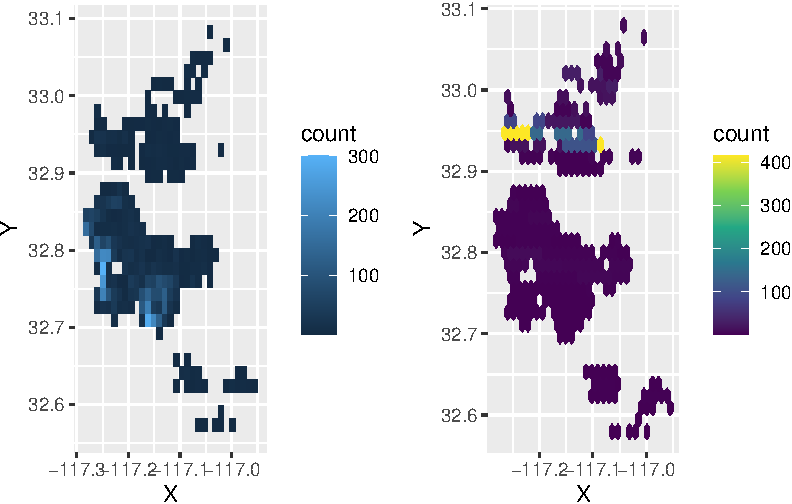
\includegraphics{02-points_files/figure-latex/unnamed-chunk-8-1.pdf}
\caption{\label{fig:unnamed-chunk-8}Raw house prices in Liverpool}
\end{figure}

This basically shows there is a lot of values concentrated around the lower end of the distribution but a few very large ones. A usual transformation to \emph{shrink} these differences is to take logarithms:

\begin{Shaded}
\begin{Highlighting}[]
\CommentTok{# Create log and add it to the table}
\NormalTok{logpr <-}\StringTok{ }\KeywordTok{log}\NormalTok{(}\KeywordTok{as.numeric}\NormalTok{(db}\OperatorTok{@}\NormalTok{data}\OperatorTok{$}\NormalTok{price))}
\NormalTok{db}\OperatorTok{@}\NormalTok{data[}\StringTok{'logpr'}\NormalTok{] <-}\StringTok{ }\NormalTok{logpr}
\CommentTok{# Create the histogram}
\NormalTok{hist <-}\StringTok{ }\KeywordTok{qplot}\NormalTok{(}\DataTypeTok{x=}\NormalTok{logpr)}
\NormalTok{hist}
\end{Highlighting}
\end{Shaded}

\begin{verbatim}
## `stat_bin()` using `bins = 30`. Pick better value with `binwidth`.
\end{verbatim}

\begin{figure}
\centering
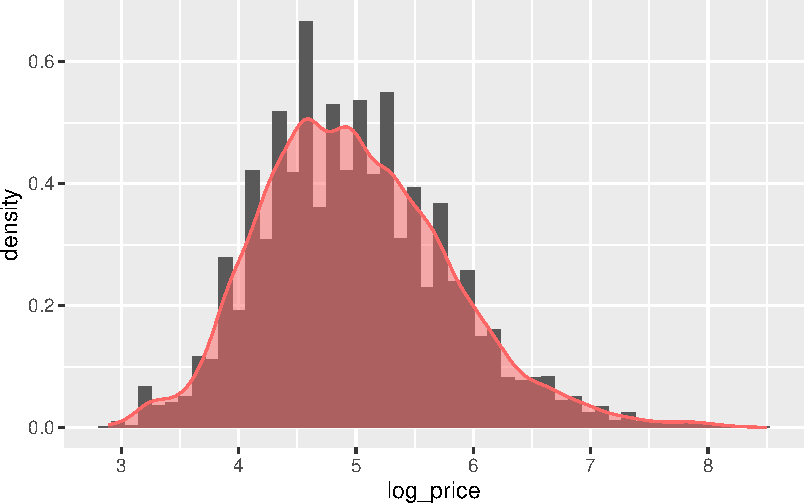
\includegraphics{02-points_files/figure-latex/unnamed-chunk-9-1.pdf}
\caption{\label{fig:unnamed-chunk-9}Log of house price in Liverpool}
\end{figure}

To obtain the spatial distribution of these houses, we need to turn away from the \texttt{@data} component of \texttt{db}. The easiest, quickest (and also dirtiest) way to get a sense of what the data look like over space is using \texttt{plot}:

\begin{Shaded}
\begin{Highlighting}[]
\KeywordTok{plot}\NormalTok{(db)}
\end{Highlighting}
\end{Shaded}

\begin{figure}
\centering
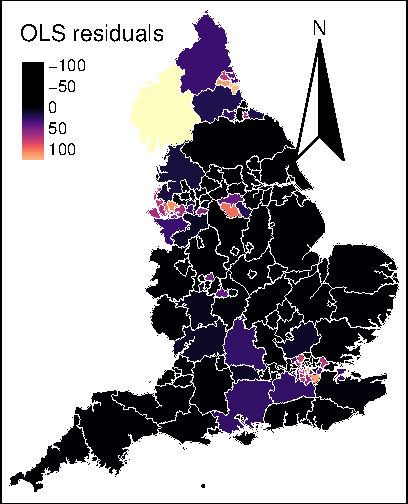
\includegraphics{02-points_files/figure-latex/unnamed-chunk-10-1.pdf}
\caption{\label{fig:unnamed-chunk-10}Spatial distribution of house transactions in Liverpool}
\end{figure}

\hypertarget{kde}{%
\section{KDE}\label{kde}}

Kernel Density Estimation (KDE) is a technique that creates a \emph{continuous} representation of the distribution of a given variable, such as house prices. Although theoretically it can be applied to any dimension, usually, KDE is applied to either one or two dimensions.

\hypertarget{one-dimensional-kde}{%
\subsection{One-dimensional KDE}\label{one-dimensional-kde}}

KDE over a single dimension is essentially a contiguous version of a histogram. We can see that by overlaying a KDE on top of the histogram of logs that we have created before:

\begin{Shaded}
\begin{Highlighting}[]
\CommentTok{# Create the base}
\NormalTok{base <-}\StringTok{ }\KeywordTok{ggplot}\NormalTok{(db}\OperatorTok{@}\NormalTok{data, }\KeywordTok{aes}\NormalTok{(}\DataTypeTok{x=}\NormalTok{logpr))}
\CommentTok{# Histogram}
\NormalTok{hist <-}\StringTok{ }\NormalTok{base }\OperatorTok{+}\StringTok{ }
\StringTok{  }\KeywordTok{geom_histogram}\NormalTok{(}\DataTypeTok{bins=}\DecValTok{50}\NormalTok{, }\KeywordTok{aes}\NormalTok{(}\DataTypeTok{y=}\NormalTok{..density..))}
\CommentTok{# Overlay density plot}
\NormalTok{kde <-}\StringTok{ }\NormalTok{hist }\OperatorTok{+}\StringTok{ }
\StringTok{  }\KeywordTok{geom_density}\NormalTok{(}\DataTypeTok{fill=}\StringTok{"#FF6666"}\NormalTok{, }\DataTypeTok{alpha=}\FloatTok{0.5}\NormalTok{, }\DataTypeTok{colour=}\StringTok{"#FF6666"}\NormalTok{)}
\NormalTok{kde}
\end{Highlighting}
\end{Shaded}

\begin{figure}
\centering
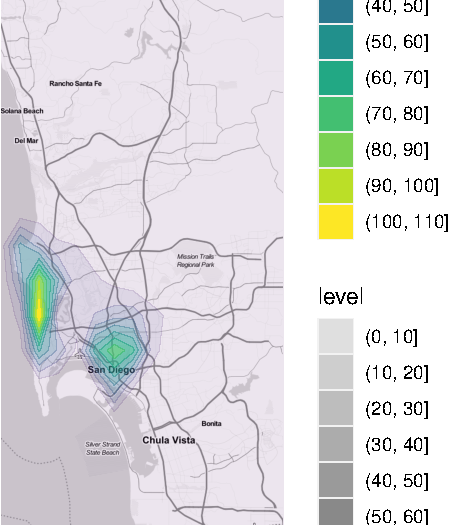
\includegraphics{02-points_files/figure-latex/unnamed-chunk-11-1.pdf}
\caption{\label{fig:unnamed-chunk-11}Histogram and KDE of the log of house prices in Liverpool}
\end{figure}

The key idea is that we are smoothing out the discrete binning that the histogram involves. Note how the histogram is exactly the same as above shape-wise, but it has been rescalend on the Y axis to reflect probabilities rather than counts.

\hypertarget{two-dimensional-spatial-kde}{%
\subsection{Two-dimensional (spatial) KDE}\label{two-dimensional-spatial-kde}}

Geography, at the end of the day, is usually represented as a two-dimensional space where we locate objects using a system of dual coordinates, \texttt{X} and \texttt{Y} (or latitude and longitude). Thanks to that, we can use the same technique as above to obtain a smooth representation of the distribution of a two-dimensional variable. The crucial difference is that, instead of obtaining a curve as the output, we will create a \emph{surface}, where intensity will be represented with a color gradient, rather than with the second dimension, as it is the case in the figure above.

To create a spatial KDE in R, there are several ways. If you do not want to necessarily acknowledge the spatial nature of your data, or you they are not stored in a spatial format, you can plot them using \texttt{ggplot2}. Note we first need to convert the coordinates (stored in the spatial part of \texttt{db}) into columns of X and Y coordinates, then we can plot them:

\begin{Shaded}
\begin{Highlighting}[]
\CommentTok{# Attach XY coordinates}
\NormalTok{db}\OperatorTok{@}\NormalTok{data[}\StringTok{'X'}\NormalTok{] <-}\StringTok{ }\NormalTok{db}\OperatorTok{@}\NormalTok{coords[, }\DecValTok{1}\NormalTok{]}
\NormalTok{db}\OperatorTok{@}\NormalTok{data[}\StringTok{'Y'}\NormalTok{] <-}\StringTok{ }\NormalTok{db}\OperatorTok{@}\NormalTok{coords[, }\DecValTok{2}\NormalTok{]}
\CommentTok{# Set up base layer}
\NormalTok{base <-}\StringTok{ }\KeywordTok{ggplot}\NormalTok{(}\DataTypeTok{data=}\NormalTok{db}\OperatorTok{@}\NormalTok{data, }\KeywordTok{aes}\NormalTok{(}\DataTypeTok{x=}\NormalTok{X, }\DataTypeTok{y=}\NormalTok{Y))}
\CommentTok{# Create the KDE surface}
\NormalTok{kde <-}\StringTok{ }\NormalTok{base }\OperatorTok{+}\StringTok{ }\KeywordTok{stat_density2d}\NormalTok{(}\KeywordTok{aes}\NormalTok{(}\DataTypeTok{x =}\NormalTok{ X, }\DataTypeTok{y =}\NormalTok{ Y, }\DataTypeTok{alpha =}\NormalTok{ ..level..), }
               \DataTypeTok{size =} \FloatTok{0.01}\NormalTok{, }\DataTypeTok{bins =} \DecValTok{16}\NormalTok{, }\DataTypeTok{geom =} \StringTok{'polygon'}\NormalTok{) }\OperatorTok{+}
\StringTok{            }\KeywordTok{scale_fill_gradient}\NormalTok{()}
\NormalTok{kde}
\end{Highlighting}
\end{Shaded}

\begin{figure}
\centering
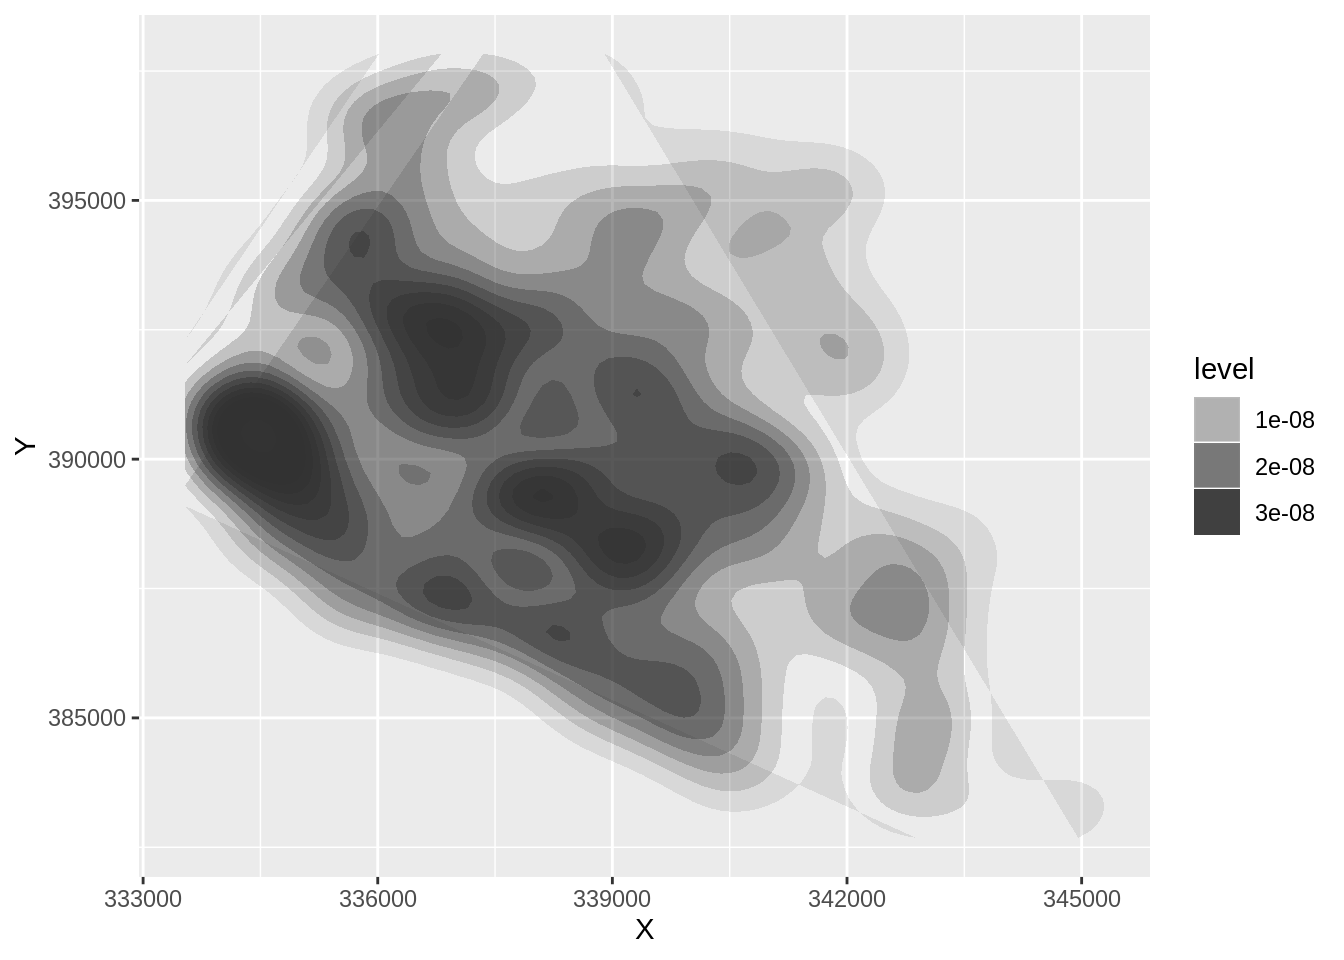
\includegraphics{02-points_files/figure-latex/unnamed-chunk-12-1.pdf}
\caption{\label{fig:unnamed-chunk-12}KDE of house transactions in Liverpool}
\end{figure}

Or, we can use a package such as the \texttt{GISTools}, which allows to pass a spatial object directly:

\begin{Shaded}
\begin{Highlighting}[]
\CommentTok{# Compute the KDE}
\NormalTok{kde <-}\StringTok{ }\KeywordTok{kde.points}\NormalTok{(db)}
\CommentTok{# Plot the KDE}
\KeywordTok{level.plot}\NormalTok{(kde)}
\end{Highlighting}
\end{Shaded}

\begin{figure}
\centering
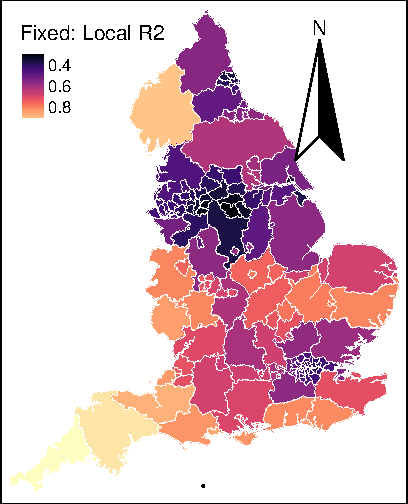
\includegraphics{02-points_files/figure-latex/unnamed-chunk-13-1.pdf}
\caption{\label{fig:unnamed-chunk-13}KDE of house transactions in Liverpool}
\end{figure}

Either of these approaches generate a surface that represents the density of dots, that is an estimation of the probability of finding a house transaction at a given coordinate. However, without any further information, they are hard to interpret and link with previous knowledge of the area. To bring such context to the figure, we can plot an underlying basemap, using a cloud provider such as Google Maps or, as in this case, OpenStreetMap. To do it, we will leverage the library \texttt{ggmap}, which is designed to play nicely with the \texttt{ggplot2} family (hence the seemingly counterintuitive example above). Before we can plot them with the online map, we need to reproject them though.

\begin{Shaded}
\begin{Highlighting}[]
\CommentTok{# Reproject coordinates}
\NormalTok{wgs84 <-}\StringTok{ }\KeywordTok{CRS}\NormalTok{(}\StringTok{"+proj=longlat +datum=WGS84 +ellps=WGS84 +towgs84=0,0,0"}\NormalTok{)}
\NormalTok{db_wgs84 <-}\StringTok{ }\KeywordTok{spTransform}\NormalTok{(db, wgs84)}
\NormalTok{db_wgs84}\OperatorTok{@}\NormalTok{data[}\StringTok{'lon'}\NormalTok{] <-}\StringTok{ }\NormalTok{db_wgs84}\OperatorTok{@}\NormalTok{coords[, }\DecValTok{1}\NormalTok{]}
\NormalTok{db_wgs84}\OperatorTok{@}\NormalTok{data[}\StringTok{'lat'}\NormalTok{] <-}\StringTok{ }\NormalTok{db_wgs84}\OperatorTok{@}\NormalTok{coords[, }\DecValTok{2}\NormalTok{]}
\NormalTok{xys <-}\StringTok{ }\NormalTok{db_wgs84}\OperatorTok{@}\NormalTok{data[}\KeywordTok{c}\NormalTok{(}\StringTok{'lon'}\NormalTok{, }\StringTok{'lat'}\NormalTok{)]}
\CommentTok{# Bounding box}
\NormalTok{liv <-}\StringTok{ }\KeywordTok{c}\NormalTok{(}\DataTypeTok{left =} \KeywordTok{min}\NormalTok{(xys}\OperatorTok{$}\NormalTok{lon), }\DataTypeTok{bottom =} \KeywordTok{min}\NormalTok{(xys}\OperatorTok{$}\NormalTok{lat), }
         \DataTypeTok{right =} \KeywordTok{max}\NormalTok{(xys}\OperatorTok{$}\NormalTok{lon), }\DataTypeTok{top =} \KeywordTok{max}\NormalTok{(xys}\OperatorTok{$}\NormalTok{lat))}
\CommentTok{# Download map tiles}
\NormalTok{basemap <-}\StringTok{ }\KeywordTok{get_stamenmap}\NormalTok{(liv, }\DataTypeTok{zoom =} \DecValTok{12}\NormalTok{, }
                         \DataTypeTok{maptype =} \StringTok{"toner-lite"}\NormalTok{)}
\end{Highlighting}
\end{Shaded}

\begin{verbatim}
## Source : http://tile.stamen.com/toner-lite/12/2013/1325.png
\end{verbatim}

\begin{verbatim}
## Source : http://tile.stamen.com/toner-lite/12/2014/1325.png
\end{verbatim}

\begin{verbatim}
## Source : http://tile.stamen.com/toner-lite/12/2015/1325.png
\end{verbatim}

\begin{verbatim}
## Source : http://tile.stamen.com/toner-lite/12/2013/1326.png
\end{verbatim}

\begin{verbatim}
## Source : http://tile.stamen.com/toner-lite/12/2014/1326.png
\end{verbatim}

\begin{verbatim}
## Source : http://tile.stamen.com/toner-lite/12/2015/1326.png
\end{verbatim}

\begin{verbatim}
## Source : http://tile.stamen.com/toner-lite/12/2013/1327.png
\end{verbatim}

\begin{verbatim}
## Source : http://tile.stamen.com/toner-lite/12/2014/1327.png
\end{verbatim}

\begin{verbatim}
## Source : http://tile.stamen.com/toner-lite/12/2015/1327.png
\end{verbatim}

\begin{Shaded}
\begin{Highlighting}[]
\CommentTok{# Overlay KDE}
\NormalTok{final <-}\StringTok{ }\KeywordTok{ggmap}\NormalTok{(basemap, }\DataTypeTok{extent =} \StringTok{"device"}\NormalTok{, }
               \DataTypeTok{maprange=}\OtherTok{FALSE}\NormalTok{) }\OperatorTok{+}
\StringTok{  }\KeywordTok{stat_density2d}\NormalTok{(}\DataTypeTok{data =}\NormalTok{ db_wgs84}\OperatorTok{@}\NormalTok{data, }
                \KeywordTok{aes}\NormalTok{(}\DataTypeTok{x =}\NormalTok{ lon, }\DataTypeTok{y =}\NormalTok{ lat, }
                    \DataTypeTok{alpha=}\NormalTok{..level.., }
                    \DataTypeTok{fill =}\NormalTok{ ..level..), }
                \DataTypeTok{size =} \FloatTok{0.01}\NormalTok{, }\DataTypeTok{bins =} \DecValTok{16}\NormalTok{, }
                \DataTypeTok{geom =} \StringTok{'polygon'}\NormalTok{, }
                \DataTypeTok{show.legend =} \OtherTok{FALSE}\NormalTok{) }\OperatorTok{+}
\StringTok{  }\KeywordTok{scale_fill_gradient2}\NormalTok{(}\StringTok{"Transaction}\CharTok{\textbackslash{}n}\StringTok{Density"}\NormalTok{, }
                       \DataTypeTok{low =} \StringTok{"#fffff8"}\NormalTok{, }
                       \DataTypeTok{high =} \StringTok{"#8da0cb"}\NormalTok{)}
\NormalTok{final}
\end{Highlighting}
\end{Shaded}

\begin{figure}
\centering
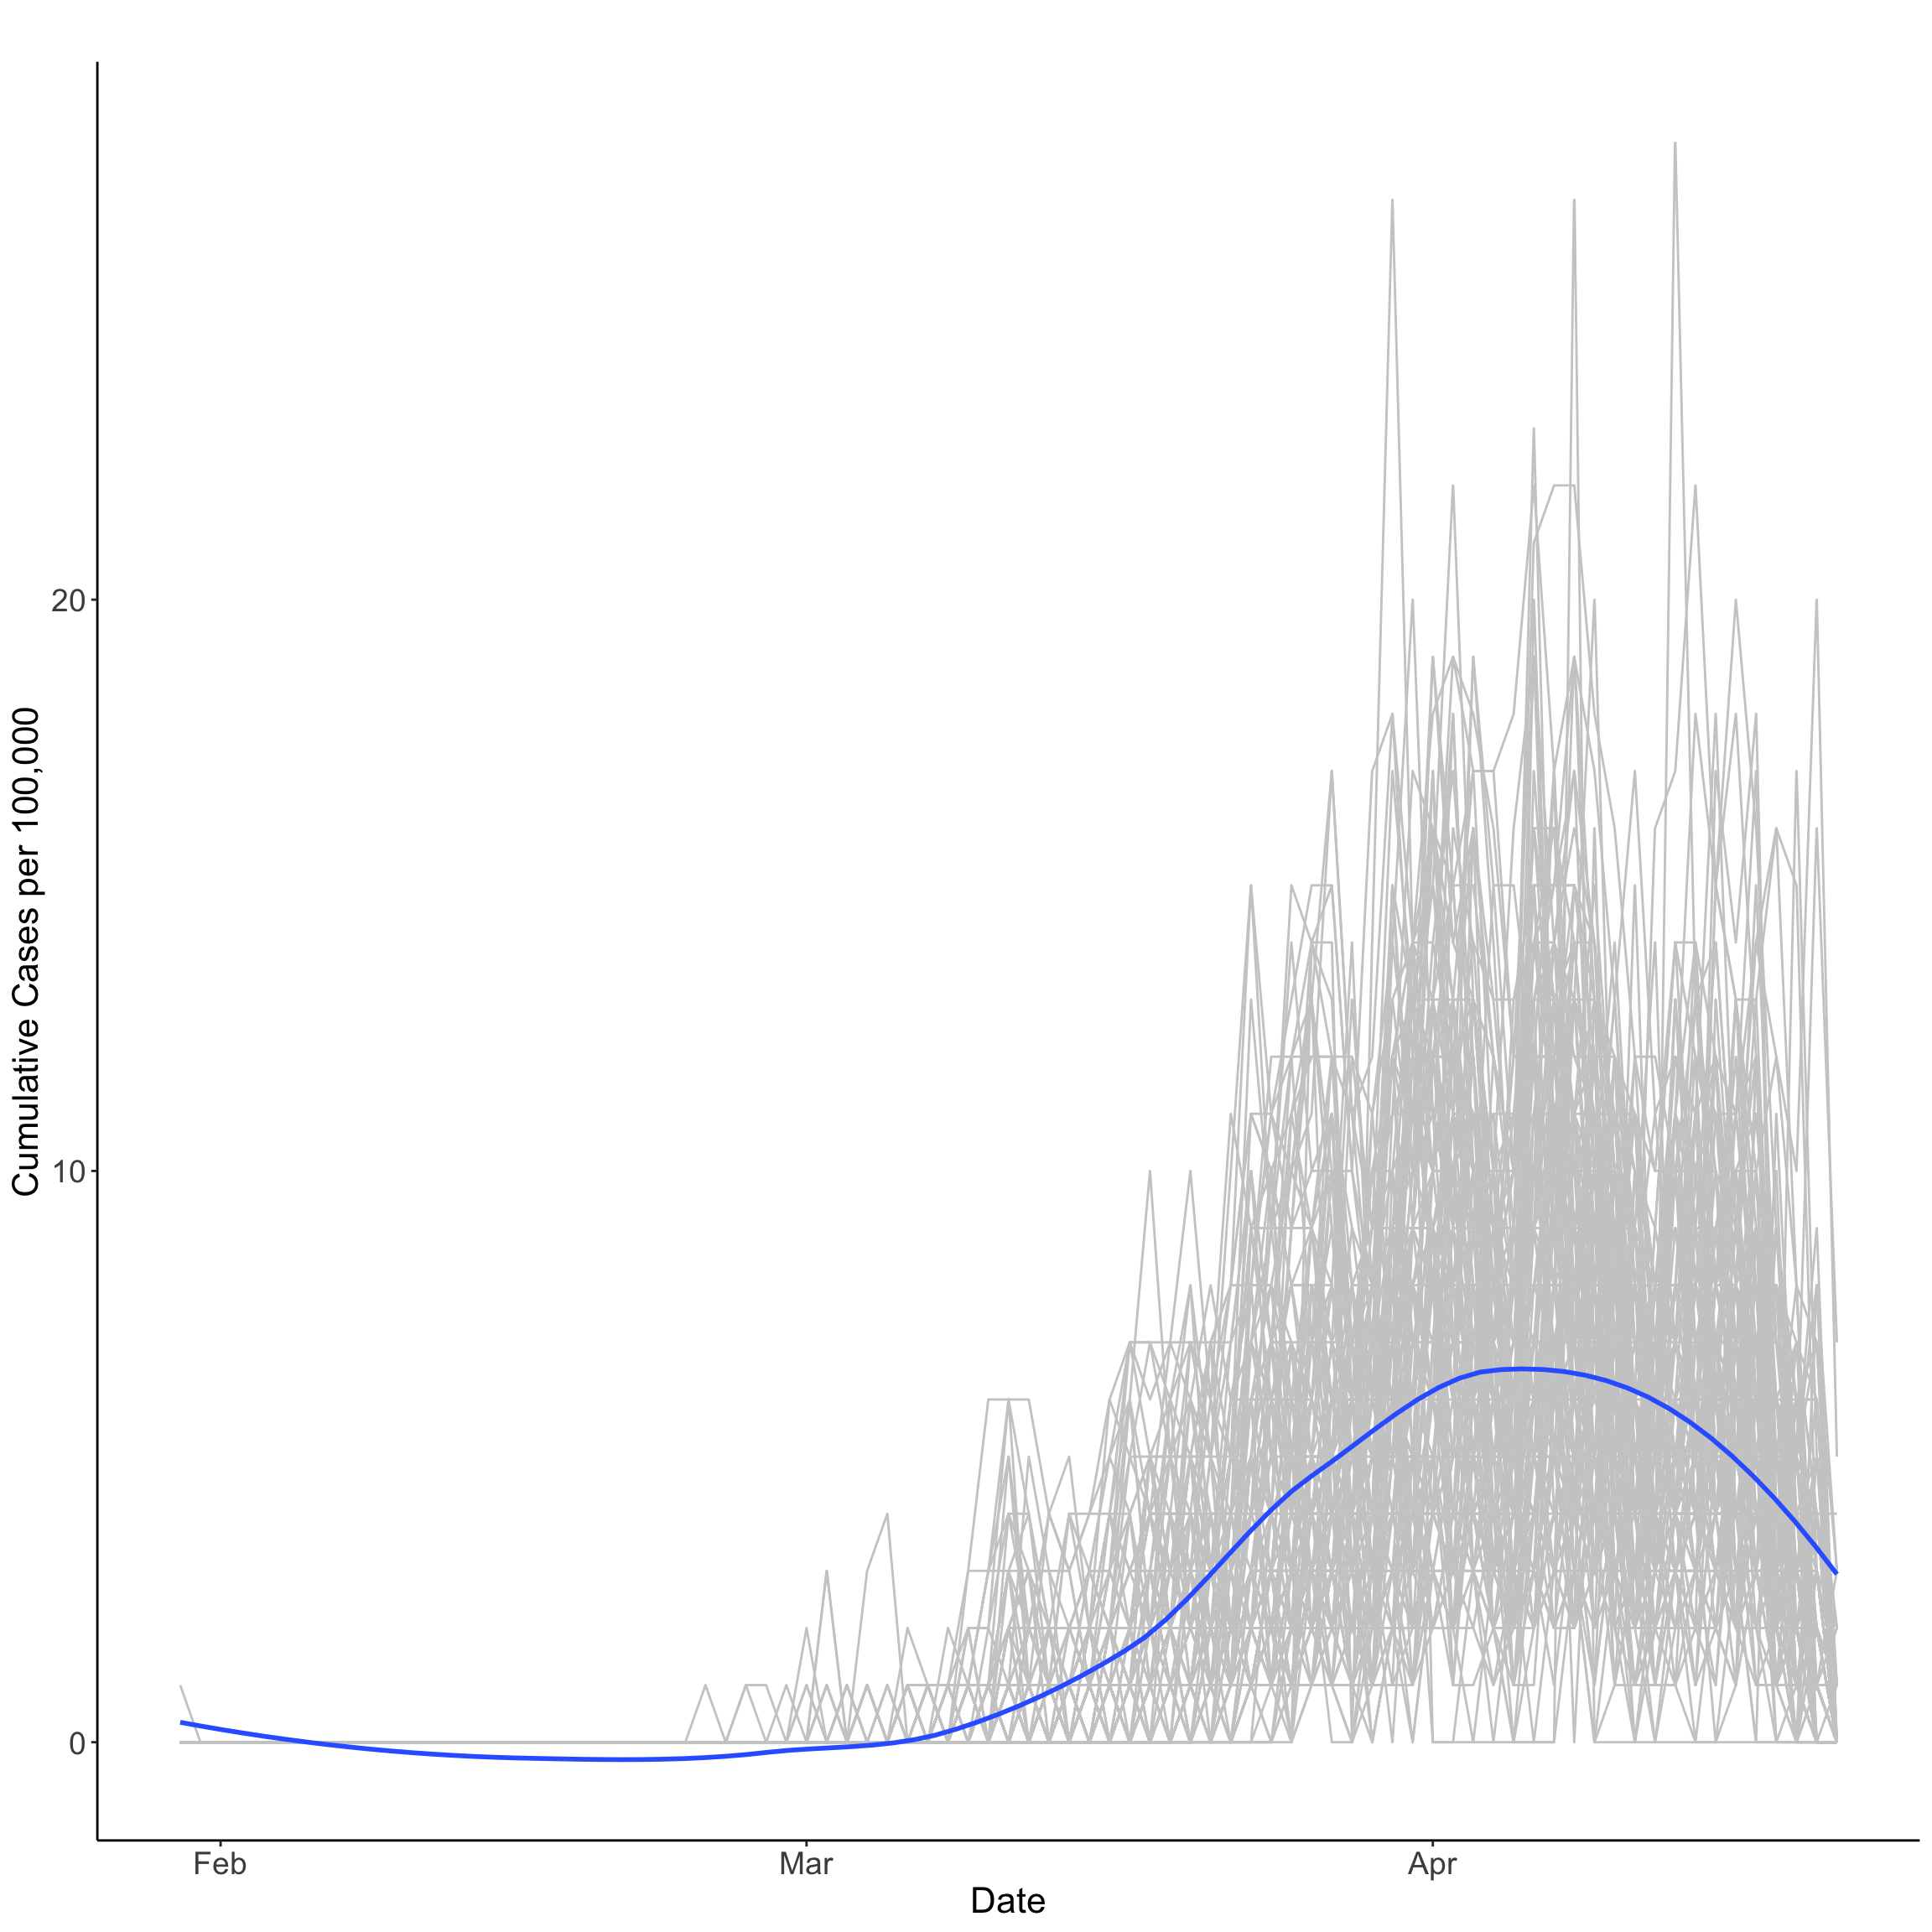
\includegraphics{02-points_files/figure-latex/unnamed-chunk-14-1.pdf}
\caption{\label{fig:unnamed-chunk-14}KDE of house transactions in Liverpool}
\end{figure}

The plot above\footnote{\textbf{EXERCISE} The map above uses the Stamen map \texttt{toner-lite}. Explore additional tile styles on their \href{http://maps.stamen.com/\#watercolor/12/37.7706/-122.3782}{website} and try to recreate the plot above.} allows us to not only see the distribution of house transactions, but to relate it to what we know about Liverpool, allowing us to establish many more connections than we were previously able. Mainly, we can easily see that the area with a highest volume of houses being sold is the city centre, with a ``hole'' around it that displays very few to no transactions and then several pockets further away.

\hypertarget{spatial-interpolation}{%
\section{Spatial Interpolation}\label{spatial-interpolation}}

The previous section demonstrates how to visualize the distribution of a set of spatial objects represented as points. In particular, given a bunch of house transactions, it shows how one can effectively visualize their distribution over space and get a sense of the density of occurrences. Such visualization, because it is based on KDE, is based on a smooth continuum, rather than on a discrete approach (as a choropleth would do, for example).

Many times however, we are not particularly interested in learning about the density of occurrences, but about the distribution of a given value attached to each location. Think for example of weather stations and temperature: the location of the stations is no secret and rarely changes, so it is not of particular interest to visualize the density of stations; what we are usually interested instead is to know how temperature is distributed over space, given we only measure it in a few places. One could argue the example we have been working with so far, house price transactions, fits into this category as well: although where house are sold may be of relevance, more often we are interested in finding out what the ``surface of price'' looks like. Rather than \emph{where are most houses being sold?} we usually want to know \emph{where the most expensive or most affordable} houses are located.

In cases where we are interested in creating a surface of a given value, rather than a simple density surface of occurrences, KDE cannot help us. In these cases, what we are interested in is \emph{spatial interpolation}, a family of techniques that aim at exactly that: creating continuous surfaces for a particular phenomenon (e.g.~temperature, house prices) given only a finite sample of observations. Spatial interpolation is a large field of research that is still being actively developed and that can involve a substantial amount of mathematical complexity in order to obtain the most accurate estimates possible\footnote{There is also an important economic incentive to do this: some of the most popular applications are in the oil and gas or mining industries. In fact, the very creator of this technique, \href{https://en.wikipedia.org/wiki/Danie_G._Krige}{Danie G. Krige}, was a mining engineer. His name is usually used to nickname spatial interpolation as \emph{kriging}.}. In this session, we will introduce the simplest possible way of interpolating values, hoping this will give you a general understanding of the methodology and, if you are interested, you can check out further literature. For example, \citet{banerjee2014hierarchical} or \citet{cressie2015statistics} are hard but good overviews.

\hypertarget{inverse-distance-weight-idw-interpolation}{%
\subsection{Inverse Distance Weight (IDW) interpolation}\label{inverse-distance-weight-idw-interpolation}}

The technique we will cover here is called \emph{Inverse Distance Weighting}, or IDW for convenience. \citet{comber2015} offer a good description:

\begin{quote}
In the \emph{inverse distance weighting} (IDW) approach to interpolation, to estimate the value of \(z\) at location \(x\) a weighted mean of nearby observations is taken {[}\ldots{]}. To accommodate the idea that observations of \(z\) at points closer to \(x\) should be given more importance in the interpolation, greater weight is given to these points {[}\ldots{]}

--- Page 204
\end{quote}

The math\footnote{Essentially, for any point \(x\) in space, the IDW estimate for value \(z\) is equivalent to \(\hat{z} (x) = \dfrac{\sum_i w_i z_i}{\sum_i w_i}\) where \(i\) are the observations for which we do have a value, and \(w_i\) is a weight given to location \(i\) based on its distance to \(x\).} is not particularly complicated and may be found in detail elsewhere (the reference above is a good starting point), so we will not spend too much time on it. More relevant in this context is the intuition behind. Essentially, the idea is that we will create a surface of house price by smoothing many values arranged along a regular grid and obtained by interpolating from the known locations to the regular grid locations. This will give us full and equal coverage to soundly perform the smoothing.

Enough chat, let's code.

From what we have just mentioned, there are a few steps to perform an IDW spatial interpolation:

\begin{enumerate}
\def\labelenumi{\arabic{enumi}.}
\tightlist
\item
  Create a regular grid over the area where we have house transactions.
\item
  Obtain IDW estimates for each point in the grid, based on the values of \(k\) nearest neighbors.
\item
  Plot a smoothed version of the grid, effectively representing the surface of house prices.
\end{enumerate}

Let us go in detail into each of them\footnote{For the relevant calculations, we will be using the \texttt{gstat} library.}. First, let us set up a grid:

\begin{Shaded}
\begin{Highlighting}[]
\NormalTok{liv.grid <-}\StringTok{ }\KeywordTok{spsample}\NormalTok{(db, }\DataTypeTok{type=}\StringTok{'regular'}\NormalTok{, }\DataTypeTok{n=}\DecValTok{25000}\NormalTok{)}
\end{Highlighting}
\end{Shaded}

That's it, we're done! The function \texttt{spsample} hugely simplifies the task by taking a spatial object and returning the grid we need. Not a couple of additional arguments we pass: \texttt{type} allows us to get a set of points that are \emph{uniformly} distributed over space, which is handy for the later smoothing; \texttt{n} controls how many points we want to create in that grid.

On to the IDW. Again, this is hugely simplified by \texttt{gstat}:

\begin{Shaded}
\begin{Highlighting}[]
\NormalTok{idw.hp <-}\StringTok{ }\KeywordTok{idw}\NormalTok{(price }\OperatorTok{~}\StringTok{ }\DecValTok{1}\NormalTok{, }\DataTypeTok{locations=}\NormalTok{db, }\DataTypeTok{newdata=}\NormalTok{liv.grid)}
\end{Highlighting}
\end{Shaded}

\begin{verbatim}
## [inverse distance weighted interpolation]
\end{verbatim}

Boom! We've got it. Let us pause for a second to see how we just did it. First, we pass \texttt{price\ \textasciitilde{}\ 1}. This specifies the formula we are using to model house prices. The name on the left of \texttt{\textasciitilde{}} represents the variable we want to explain, while everything to its right captures the \emph{explanatory} variables. Since we are considering the simplest possible case, we do not have further variables to add, so we simply write \texttt{1}. Then we specify the original locations for which we do have house prices (our original \texttt{db} object), and the points where we want to interpolate the house prices (the \texttt{liv.grid} object we just created above). One more note: by default, \texttt{idw.hp} uses all the available observations, weighted by distance, to provide an estimate for a given point. If you want to modify that and restrict the maximum number of neighbors to consider, you need to tweak the argument \texttt{nmax}, as we do above by using the 150 neares observations to each point\footnote{Have a play with this because the results do change significantly. Can you reason why?}.

The object we get from \texttt{idw} is another spatial table, just as \texttt{db}, containing the interpolated values. As such, we can inspect it just as with any other of its kind. For example, to check out the top of the estimated table:

\begin{Shaded}
\begin{Highlighting}[]
\KeywordTok{head}\NormalTok{(idw.hp}\OperatorTok{@}\NormalTok{data)}
\end{Highlighting}
\end{Shaded}

\begin{verbatim}
##   var1.pred var1.var
## 1  158044.8       NA
## 2  158154.3       NA
## 3  158266.6       NA
## 4  158381.8       NA
## 5  158499.9       NA
## 6  158621.1       NA
\end{verbatim}

The column we will pay attention to is \texttt{var1.pred}. And to see the locations for which those correspond:

\begin{Shaded}
\begin{Highlighting}[]
\KeywordTok{head}\NormalTok{(idw.hp}\OperatorTok{@}\NormalTok{coords)}
\end{Highlighting}
\end{Shaded}

\begin{verbatim}
##            x1       x2
## [1,] 333555.0 382714.2
## [2,] 333640.0 382714.2
## [3,] 333724.9 382714.2
## [4,] 333809.9 382714.2
## [5,] 333894.8 382714.2
## [6,] 333979.8 382714.2
\end{verbatim}

So, for a hypothetical house sold at the location in the first row of \texttt{idw.hp@coords} (expressed in the OSGB coordinate system), the price we would guess it would cost, based on the price of houses sold nearby, is the first element of column \texttt{var1.pred} in \texttt{idw.hp@data}.

\hypertarget{a-surface-of-housing-prices}{%
\subsection{A surface of housing prices}\label{a-surface-of-housing-prices}}

Once we have the IDW object computed, we can plot it to explore the distribution, not of house transactions in this case, but of house price over the geography of Liverpool. The easiest way to do this is by quickly calling the command \texttt{spplot}:

\begin{Shaded}
\begin{Highlighting}[]
\KeywordTok{spplot}\NormalTok{(idw.hp[}\StringTok{'var1.pred'}\NormalTok{])}
\end{Highlighting}
\end{Shaded}

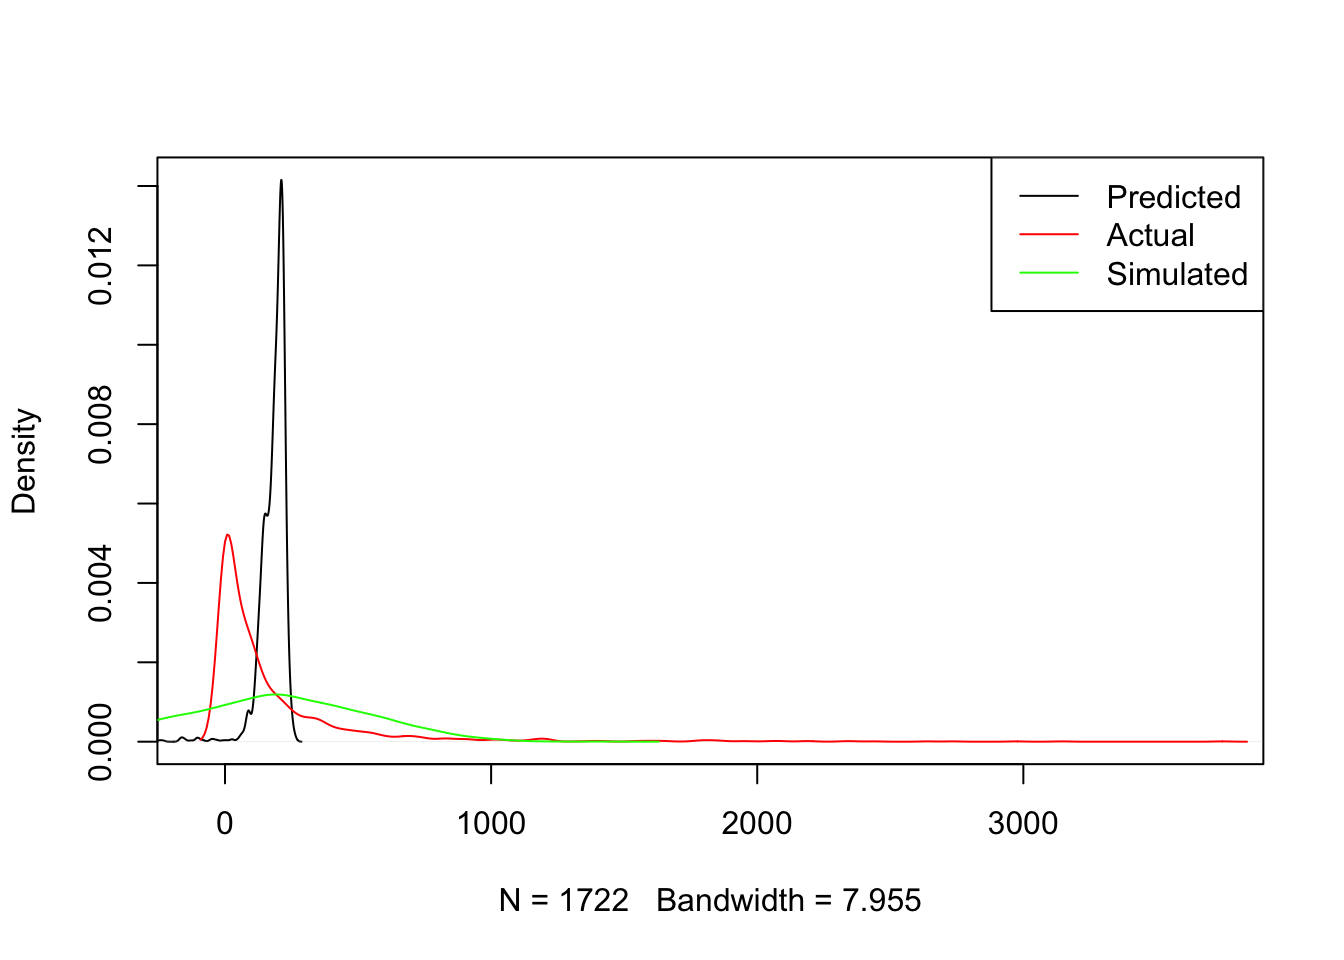
\includegraphics{02-points_files/figure-latex/unnamed-chunk-19-1.pdf}

However, this is not entirely satisfactory for a number of reasons. Let us get an equivalen plot with the package \texttt{tmap}, which streamlines some of this and makes more aesthetically pleasant maps easier to build as it follows a ``ggplot-y'' approach.

\begin{Shaded}
\begin{Highlighting}[]
\CommentTok{# Load up the layer}
\NormalTok{liv.otl <-}\StringTok{ }\KeywordTok{readOGR}\NormalTok{(}\StringTok{'data/house_transactions'}\NormalTok{, }\StringTok{'liv_outline'}\NormalTok{)}
\end{Highlighting}
\end{Shaded}

\begin{verbatim}
## OGR data source with driver: ESRI Shapefile 
## Source: "/home/jovyan/work/data/house_transactions", layer: "liv_outline"
## with 1 features
## It has 1 fields
\end{verbatim}

The shape we will overlay looks like this:

\begin{Shaded}
\begin{Highlighting}[]
\KeywordTok{qtm}\NormalTok{(liv.otl)}
\end{Highlighting}
\end{Shaded}

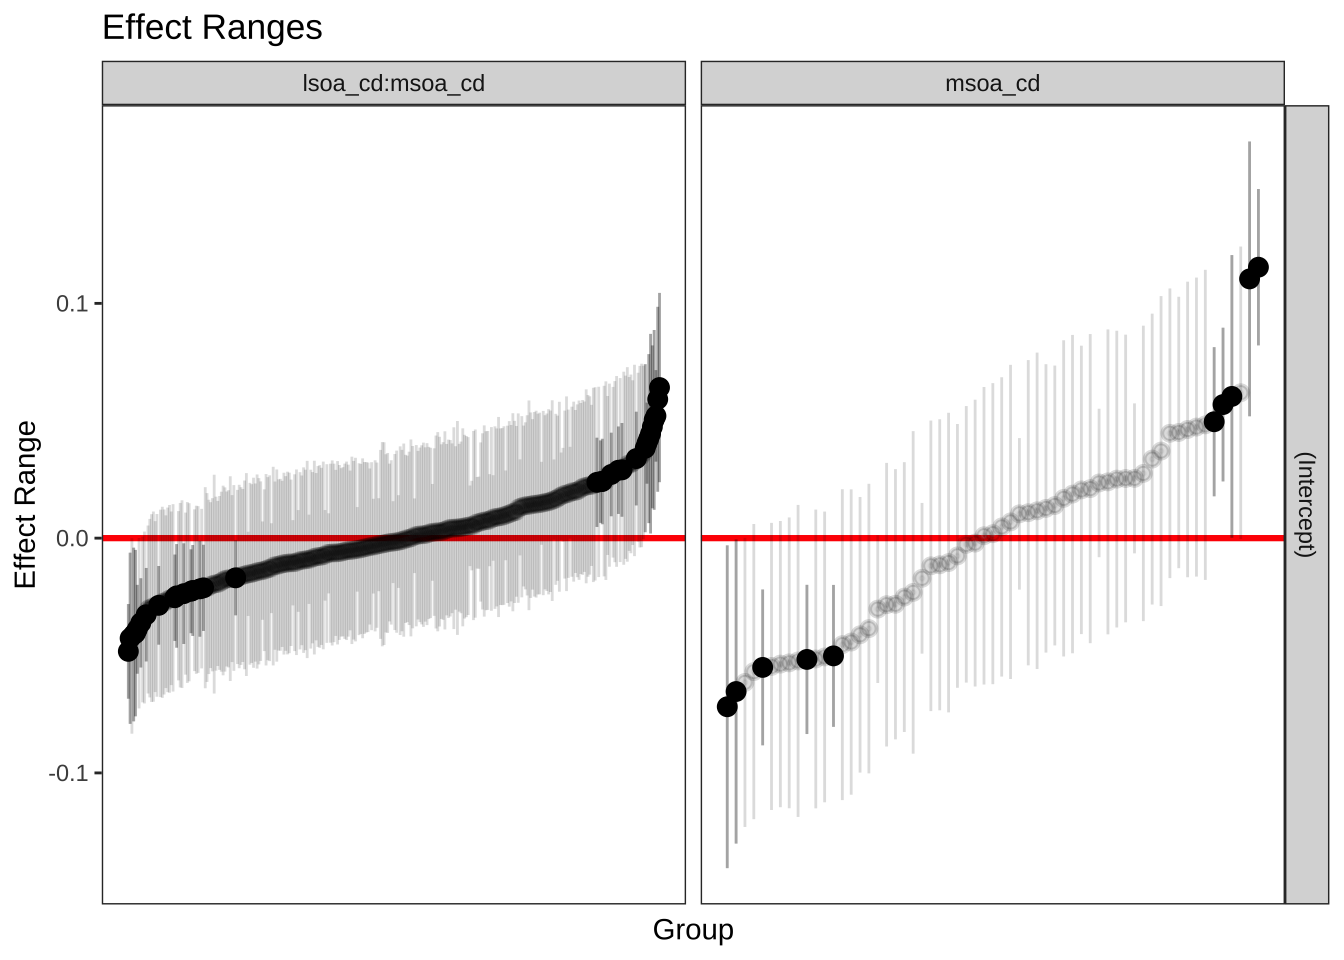
\includegraphics{02-points_files/figure-latex/unnamed-chunk-21-1.pdf}

Now let's give it a first go!

\begin{Shaded}
\begin{Highlighting}[]
\CommentTok{# }
\NormalTok{p =}\StringTok{ }\KeywordTok{tm_shape}\NormalTok{(liv.otl) }\OperatorTok{+}\StringTok{ }\KeywordTok{tm_fill}\NormalTok{(}\DataTypeTok{col=}\StringTok{'black'}\NormalTok{, }\DataTypeTok{alpha=}\DecValTok{1}\NormalTok{) }\OperatorTok{+}
\StringTok{  }\KeywordTok{tm_shape}\NormalTok{(idw.hp) }\OperatorTok{+}\StringTok{ }
\StringTok{  }\KeywordTok{tm_symbols}\NormalTok{(}\DataTypeTok{col=}\StringTok{'var1.pred'}\NormalTok{, }\DataTypeTok{size=}\FloatTok{0.1}\NormalTok{, }\DataTypeTok{alpha=}\FloatTok{0.25}\NormalTok{, }
             \DataTypeTok{border.lwd=}\FloatTok{0.}\NormalTok{, }\DataTypeTok{palette=}\StringTok{'YlGn'}\NormalTok{)}
\NormalTok{p}
\end{Highlighting}
\end{Shaded}

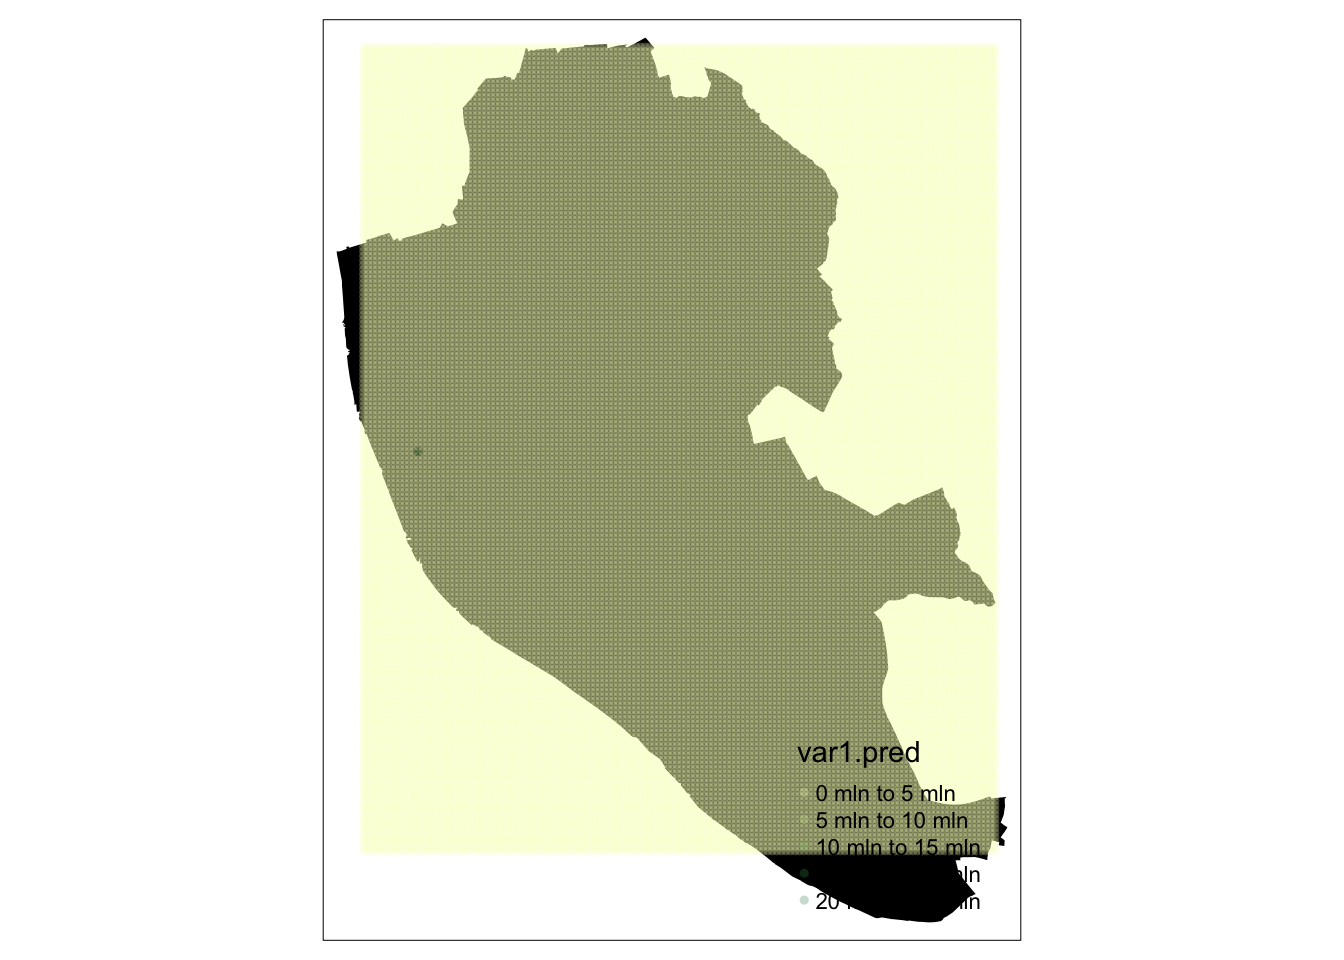
\includegraphics{02-points_files/figure-latex/unnamed-chunk-22-1.pdf}

The last two plots, however, are not really a surface, but a representation of the points we have just estimated. To create a surface, we need to do an interim transformation to convert the spatial object \texttt{idw.hp} into a table that a ``surface plotter'' can understand.

\begin{Shaded}
\begin{Highlighting}[]
\NormalTok{xyz <-}\StringTok{ }\KeywordTok{data.frame}\NormalTok{(}\DataTypeTok{x=}\KeywordTok{coordinates}\NormalTok{(idw.hp)[, }\DecValTok{1}\NormalTok{], }
                  \DataTypeTok{y=}\KeywordTok{coordinates}\NormalTok{(idw.hp)[, }\DecValTok{2}\NormalTok{], }
                  \DataTypeTok{z=}\NormalTok{idw.hp}\OperatorTok{$}\NormalTok{var1.pred)}
\end{Highlighting}
\end{Shaded}

Now we are ready to plot the surface as a contour:

\begin{Shaded}
\begin{Highlighting}[]
\NormalTok{base <-}\StringTok{ }\KeywordTok{ggplot}\NormalTok{(}\DataTypeTok{data=}\NormalTok{xyz, }\KeywordTok{aes}\NormalTok{(}\DataTypeTok{x=}\NormalTok{x, }\DataTypeTok{y=}\NormalTok{y))}
\NormalTok{surface <-}\StringTok{ }\NormalTok{base }\OperatorTok{+}\StringTok{ }\KeywordTok{geom_contour}\NormalTok{(}\KeywordTok{aes}\NormalTok{(}\DataTypeTok{z=}\NormalTok{z))}
\NormalTok{surface}
\end{Highlighting}
\end{Shaded}

\begin{figure}
\centering
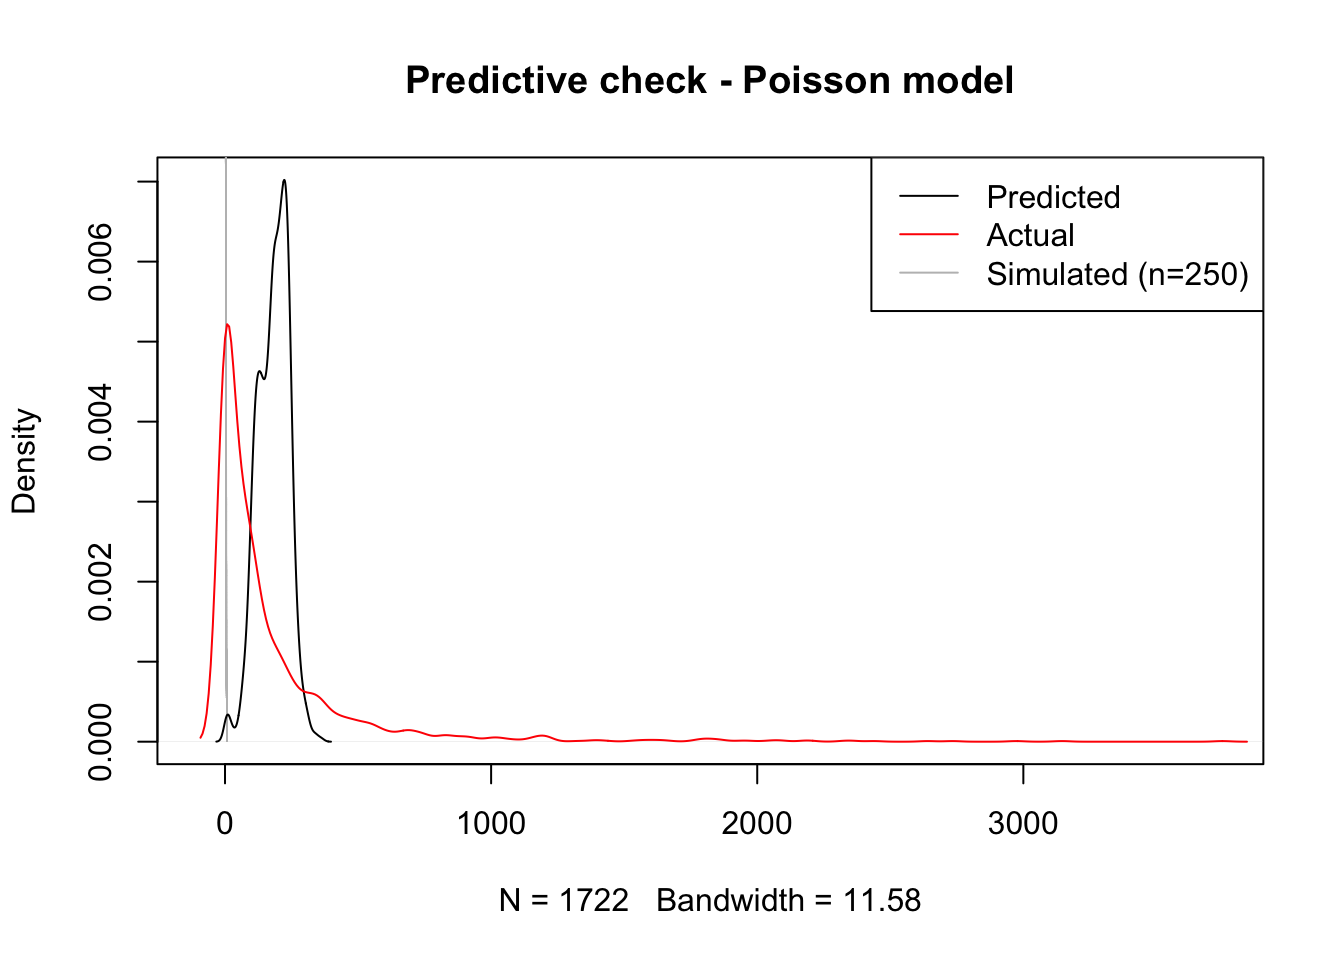
\includegraphics{02-points_files/figure-latex/unnamed-chunk-24-1.pdf}
\caption{\label{fig:unnamed-chunk-24}Contour of prices in Liverpool}
\end{figure}

Which can also be shown as a filled contour:

\begin{Shaded}
\begin{Highlighting}[]
\NormalTok{base <-}\StringTok{ }\KeywordTok{ggplot}\NormalTok{(}\DataTypeTok{data=}\NormalTok{xyz, }\KeywordTok{aes}\NormalTok{(}\DataTypeTok{x=}\NormalTok{x, }\DataTypeTok{y=}\NormalTok{y))}
\NormalTok{surface <-}\StringTok{ }\NormalTok{base }\OperatorTok{+}\StringTok{ }\KeywordTok{geom_raster}\NormalTok{(}\KeywordTok{aes}\NormalTok{(}\DataTypeTok{fill=}\NormalTok{z))}
\NormalTok{surface}
\end{Highlighting}
\end{Shaded}

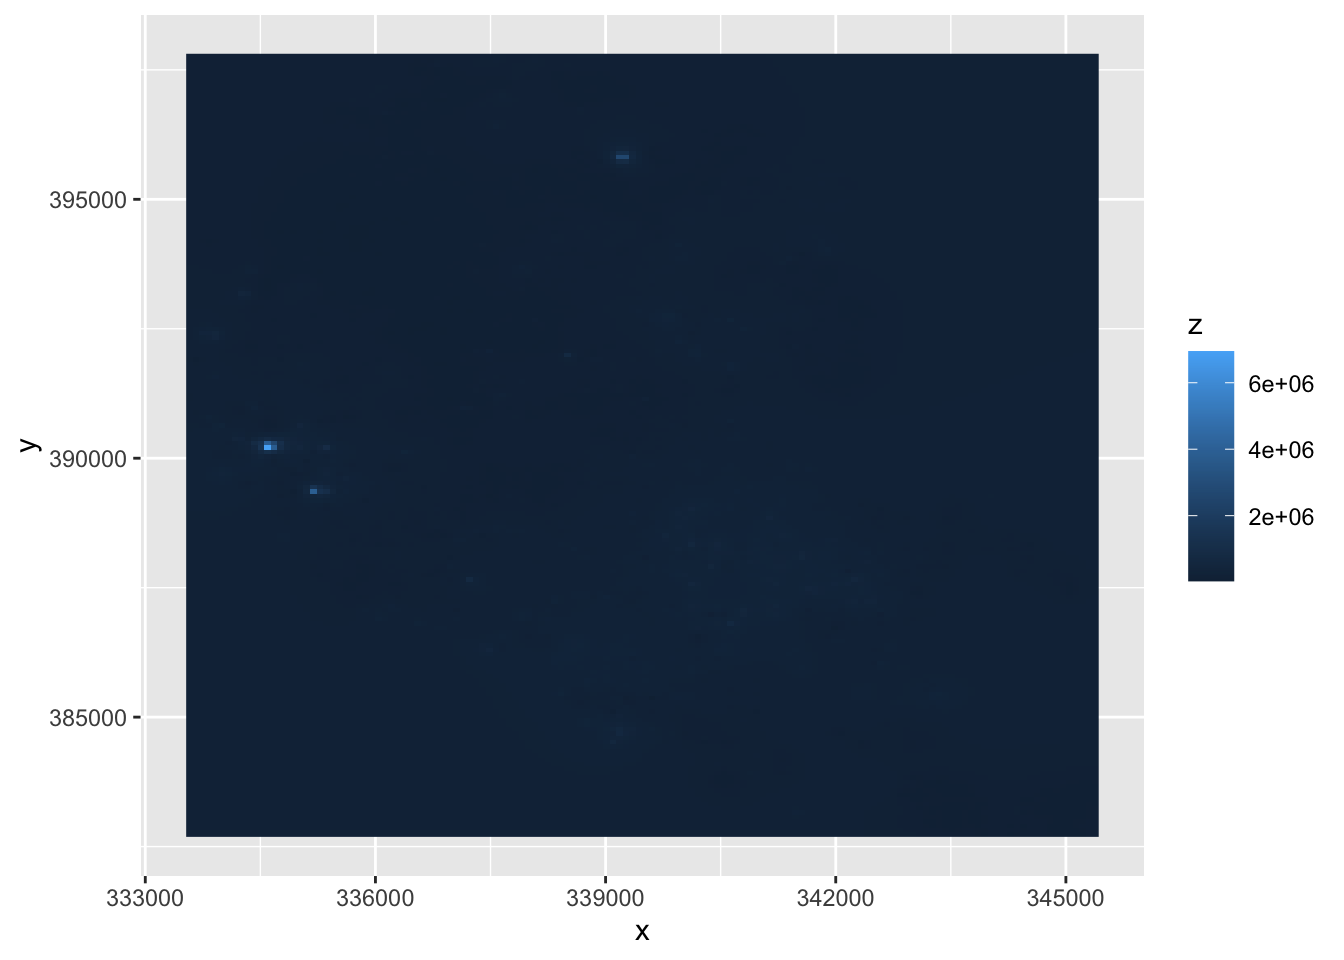
\includegraphics{02-points_files/figure-latex/unnamed-chunk-25-1.pdf}

The problem here, when compared to the KDE above for example, is that a few values are extremely large:

\begin{Shaded}
\begin{Highlighting}[]
\KeywordTok{qplot}\NormalTok{(}\DataTypeTok{data=}\NormalTok{xyz, }\DataTypeTok{x=}\NormalTok{z, }\DataTypeTok{geom=}\StringTok{'density'}\NormalTok{)}
\end{Highlighting}
\end{Shaded}

\begin{figure}
\centering
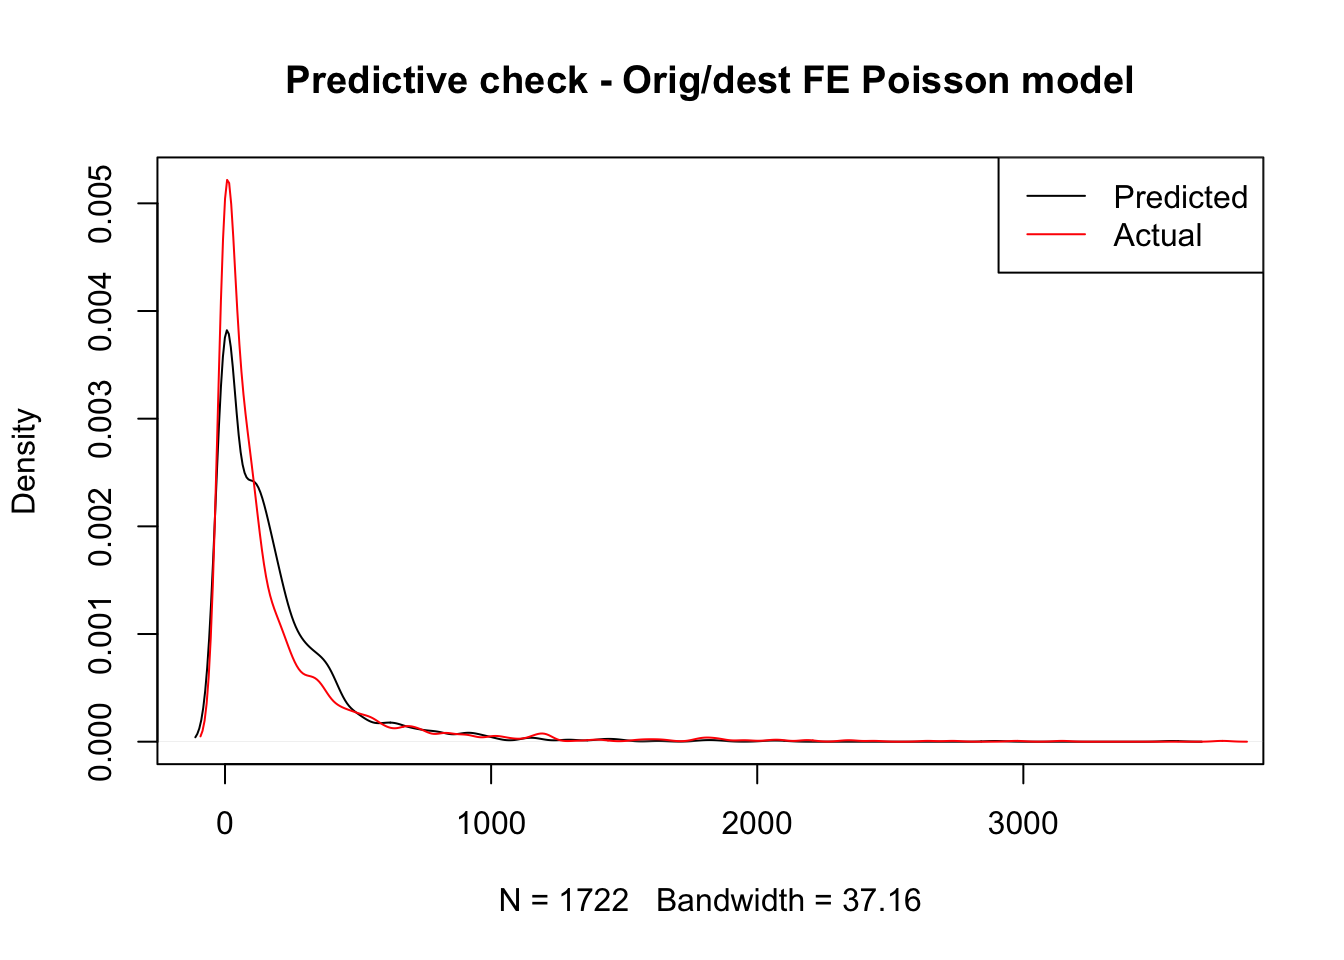
\includegraphics{02-points_files/figure-latex/unnamed-chunk-26-1.pdf}
\caption{\label{fig:unnamed-chunk-26}Skewness of prices in Liverpool}
\end{figure}

Let us then take the logarithm before we plot the surface:

\begin{Shaded}
\begin{Highlighting}[]
\NormalTok{xyz[}\StringTok{'lz'}\NormalTok{] <-}\StringTok{ }\KeywordTok{log}\NormalTok{(xyz}\OperatorTok{$}\NormalTok{z)}
\NormalTok{base <-}\StringTok{ }\KeywordTok{ggplot}\NormalTok{(}\DataTypeTok{data=}\NormalTok{xyz, }\KeywordTok{aes}\NormalTok{(}\DataTypeTok{x=}\NormalTok{x, }\DataTypeTok{y=}\NormalTok{y))}
\NormalTok{surface <-}\StringTok{ }\NormalTok{base }\OperatorTok{+}
\StringTok{           }\KeywordTok{geom_raster}\NormalTok{(}\KeywordTok{aes}\NormalTok{(}\DataTypeTok{fill=}\NormalTok{lz),}
                       \DataTypeTok{show.legend =}\NormalTok{ F)}
\NormalTok{surface}
\end{Highlighting}
\end{Shaded}

\begin{figure}
\centering
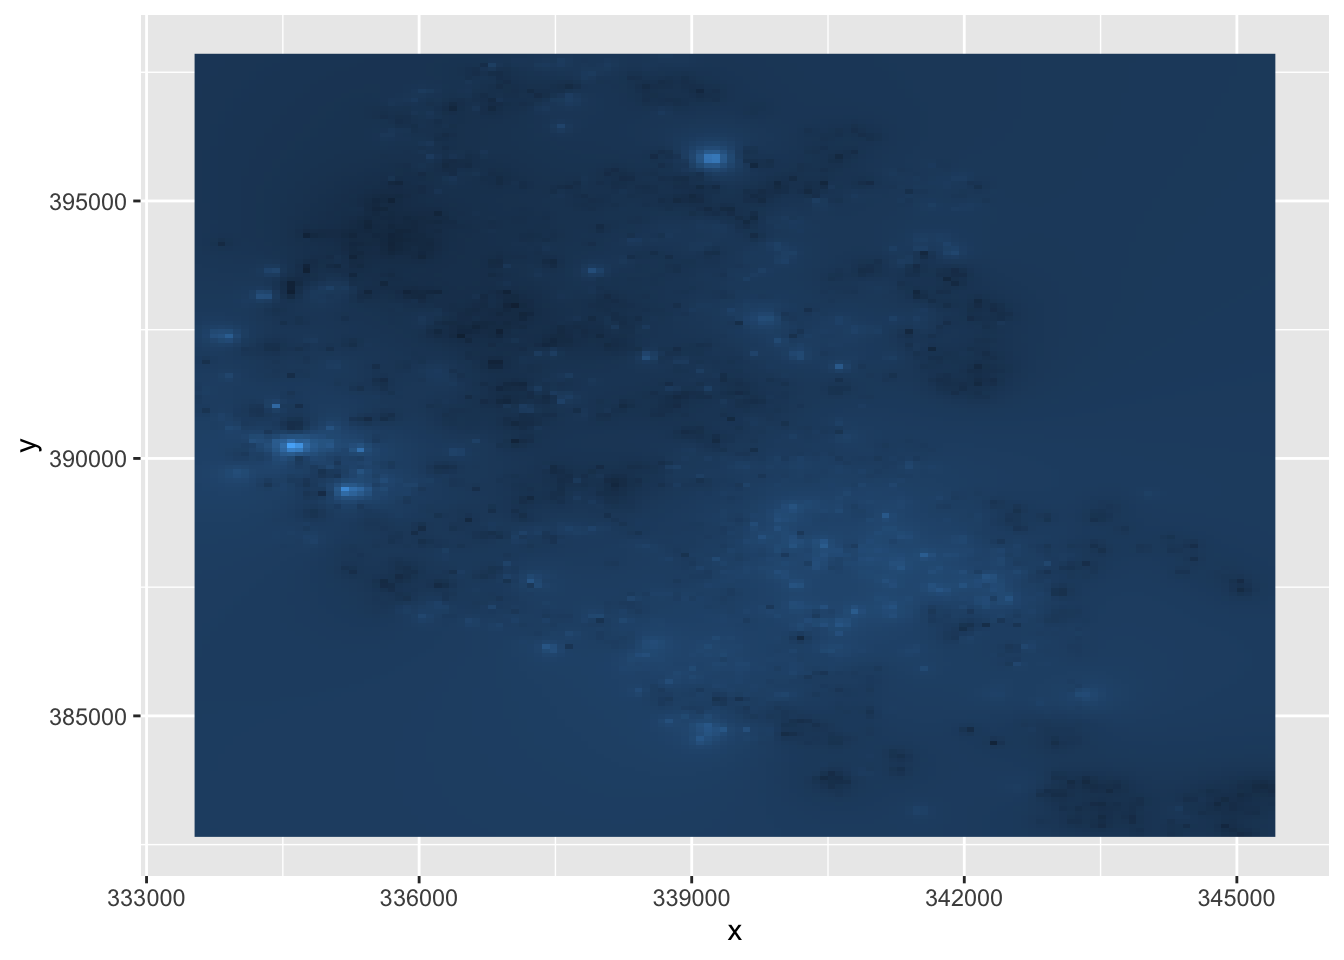
\includegraphics{02-points_files/figure-latex/unnamed-chunk-27-1.pdf}
\caption{\label{fig:unnamed-chunk-27}Surface of log-prices in Liverpool}
\end{figure}

Now this looks better. We can start to tell some patterns. To bring in context, it would be great to be able to add a basemap layer, as we did for the KDE. This is conceptually very similar to what we did above, starting by reprojecting the points and continuing by overlaying them on top of the basemap. However, technically speaking it is not possible because \texttt{ggmap} --the library we have been using to display tiles from cloud providers-- does not play well with our own rasters (i.e.~the price surface). At the moment, it is surprisingly tricky to get this to work, so we will park it for now. However, developments such as the \href{https://github.com/edzer/sfr}{\texttt{sf}} project promise to make this easier in the future\footnote{\textbf{BONUS} if you can figure out a way to do it yourself!}.

\hypertarget{what-should-the-next-houses-price-be}{%
\subsection{\texorpdfstring{\emph{``What should the next house's price be?''}}{``What should the next house's price be?''}}\label{what-should-the-next-houses-price-be}}

The last bit we will explore in this session relates to prediction for new values. Imagine you are a real state data scientist and your boss asks you to give an estimate of how much a new house going into the market should cost. The only information you have to make such a guess is the location of the house. In this case, the IDW model we have just fitted can help you. The trick is realizing that, instead of creating an entire grid, all we need is to obtain an estimate of a single location.

Let us say, the house is located on the coordinates \texttt{x=340000,\ y=390000} as expressed in the GB National Grid coordinate system. In that case, we can do as follows:

\begin{Shaded}
\begin{Highlighting}[]
\NormalTok{pt <-}\StringTok{ }\KeywordTok{SpatialPoints}\NormalTok{(}\KeywordTok{cbind}\NormalTok{(}\DataTypeTok{x=}\DecValTok{340000}\NormalTok{, }\DataTypeTok{y=}\DecValTok{390000}\NormalTok{),}
                    \DataTypeTok{proj4string =}\NormalTok{ db}\OperatorTok{@}\NormalTok{proj4string)}
\NormalTok{idw.one <-}\StringTok{ }\KeywordTok{idw}\NormalTok{(price }\OperatorTok{~}\StringTok{ }\DecValTok{1}\NormalTok{, }\DataTypeTok{locations=}\NormalTok{db, }\DataTypeTok{newdata=}\NormalTok{pt)}
\end{Highlighting}
\end{Shaded}

\begin{verbatim}
## [inverse distance weighted interpolation]
\end{verbatim}

\begin{Shaded}
\begin{Highlighting}[]
\NormalTok{idw.one}
\end{Highlighting}
\end{Shaded}

\begin{verbatim}
## class       : SpatialPointsDataFrame 
## features    : 1 
## extent      : 340000, 340000, 390000, 390000  (xmin, xmax, ymin, ymax)
## crs         : +proj=tmerc +lat_0=49 +lon_0=-2 +k=0.9996012717 +x_0=400000 +y_0=-100000 +datum=OSGB36 +units=m +no_defs +ellps=airy +towgs84=446.448,-125.157,542.060,0.1502,0.2470,0.8421,-20.4894 
## variables   : 2
## names       :        var1.pred, var1.var 
## value       : 157099.029513871,       NA
\end{verbatim}

And, as show above, the estimated value is GBP157,099\footnote{\textbf{PRO QUESTION} Is that house expensive or cheap, as compared to the other houses sold in this dataset? Can you figure out where the house is?}.

Using this predictive logic, and taking advantage of Google Maps and its geocoding capabilities, it is possible to devise a function that takes an arbitrary address in Liverpool and, based on the transactions occurred throughout 2014, provides an estimate of what the price for a property in that location could be.

\begin{Shaded}
\begin{Highlighting}[]
\NormalTok{how.much.is <-}\StringTok{ }\ControlFlowTok{function}\NormalTok{(address, }\DataTypeTok{print.message=}\OtherTok{TRUE}\NormalTok{)\{}
  \CommentTok{# Convert the address into Lon/Lat coordinates}
  \CommentTok{# }\AlertTok{NOTE}\CommentTok{: this now requires an API key}
  \CommentTok{# https://github.com/dkahle/ggmap#google-maps-and-credentials}
\NormalTok{  ll.pt <-}\StringTok{ }\KeywordTok{geocode}\NormalTok{(address)}
  \CommentTok{# Process as spatial table}
\NormalTok{  wgs84 <-}\StringTok{ }\KeywordTok{CRS}\NormalTok{(}\StringTok{"+proj=longlat +datum=WGS84 +ellps=WGS84 +towgs84=0,0,0"}\NormalTok{)}
\NormalTok{  ll.pt <-}\StringTok{ }\KeywordTok{SpatialPoints}\NormalTok{(}\KeywordTok{cbind}\NormalTok{(}\DataTypeTok{x=}\NormalTok{ll.pt}\OperatorTok{$}\NormalTok{lon, }\DataTypeTok{y=}\NormalTok{ll.pt}\OperatorTok{$}\NormalTok{lat),}
                      \DataTypeTok{proj4string =}\NormalTok{ wgs84)}
  \CommentTok{# Transform Lon/Lat into OSGB}
\NormalTok{  pt <-}\StringTok{ }\KeywordTok{spTransform}\NormalTok{(ll.pt, db}\OperatorTok{@}\NormalTok{proj4string)}
  \CommentTok{# Obtain prediction}
\NormalTok{  idw.one <-}\StringTok{ }\KeywordTok{idw}\NormalTok{(price }\OperatorTok{~}\StringTok{ }\DecValTok{1}\NormalTok{, }\DataTypeTok{locations=}\NormalTok{db, }\DataTypeTok{newdata=}\NormalTok{pt)}
\NormalTok{  price <-}\StringTok{ }\NormalTok{idw.one}\OperatorTok{@}\NormalTok{data}\OperatorTok{$}\NormalTok{var1.pred}
  \CommentTok{# Return predicted price}
  \ControlFlowTok{if}\NormalTok{(print.message}\OperatorTok{==}\NormalTok{T)\{}
    \KeywordTok{writeLines}\NormalTok{(}\KeywordTok{paste}\NormalTok{(}\StringTok{"}\CharTok{\textbackslash{}n\textbackslash{}n}\StringTok{Based on what surrounding properties were sold"}\NormalTok{,}
                    \StringTok{"for in 2014 a house located at"}\NormalTok{, address, }\StringTok{"would"}\NormalTok{, }
                    \StringTok{"cost"}\NormalTok{,  }\KeywordTok{paste}\NormalTok{(}\StringTok{"GBP"}\NormalTok{, }\KeywordTok{round}\NormalTok{(price), }\StringTok{"."}\NormalTok{, }\DataTypeTok{sep=}\StringTok{''}\NormalTok{), }\StringTok{"}\CharTok{\textbackslash{}n\textbackslash{}n}\StringTok{"}\NormalTok{))}
\NormalTok{  \}}
  \KeywordTok{return}\NormalTok{(price)}
\NormalTok{\}}
\end{Highlighting}
\end{Shaded}

Ready to test!

\begin{Shaded}
\begin{Highlighting}[]
\NormalTok{address <-}\StringTok{ "74 Bedford St S, Liverpool, L69 7ZT, UK"}
\CommentTok{#p <- how.much.is(address)}
\end{Highlighting}
\end{Shaded}

\hypertarget{flows}{%
\chapter{Flows}\label{flows}}

DA-B to fill in

\hypertarget{spatial-econometrics}{%
\chapter{Spatial Econometrics}\label{spatial-econometrics}}

DA-B to fill in

\hypertarget{multilevel-models-pt.-i}{%
\chapter{Multilevel Models (Pt. I)}\label{multilevel-models-pt.-i}}

FR-G to fill in

\hypertarget{multilevel-models-pt.-ii}{%
\chapter{Multilevel Models (Pt. II)}\label{multilevel-models-pt.-ii}}

FR-G to fill in

\hypertarget{gwr}{%
\chapter{GWR}\label{gwr}}

FR-G

\hypertarget{space-time-analysis}{%
\chapter{Space-Time Analysis}\label{space-time-analysis}}

FR-G

\bibliography{book.bib,packages.bib}


\end{document}
